\documentclass[12pt]{article}% 这是主要的格式。
\usepackage[UTF8]{ctex}
\usepackage[page,title,titletoc,header]{appendix}
\usepackage{enumerate}
\usepackage{amsmath}
\usepackage{graphicx}
 \usepackage{listings}
\usepackage{autobreak}
 \usepackage{textcomp} % 必须加上,否则报错
 \usepackage[framed,numbered,autolinebreaks,useliterate]{mcode}
 \usepackage{xcolor}
 \usepackage{longtable}
 \lstset{numbers=left, numberstyle= \tiny, escapeinside=``}
\usepackage[labelsep=space]{caption}
\usepackage{cite}
\usepackage{textcomp}
\usepackage{array}
\usepackage{multirow}
\usepackage{bigstrut}
\usepackage{geometry}
\usepackage{graphicx}
\usepackage{subcaption}
\usepackage[framed,numbered,autolinebreaks,useliterate]{mcode}
\geometry{left =2.5 cm,right=2.5cm,top=2.5cm,bottom=2.5cm}
\usepackage[section]{placeins}
\usepackage[colorlinks,linkcolor=black,citecolor=black]{hyperref}
\usepackage{titlesec}
\usepackage{titletoc}
\titleformat{\section}{\heiti\zihao{4}}{\thesection}{0.3em}{}
\titleformat{\subsection}{\heiti \fontsize{12pt}{0}}{\thesubsection}{0.3em}{}
\titleformat{\subsubsection}{\heiti \fontsize{12pt}{0}}{\thesubsubsection}{0.3em}{}
\renewcommand{\contentsname}{\songti\centerline{目录}}
\renewcommand\figurename{\heiti\zihao{5} 图}
\renewcommand\tablename{\heiti\zihao{5} 表}
\title{ \heiti\zihao{3}}
\author{}
\date{}

\begin{document}
\thispagestyle{empty}
\tableofcontents
\thispagestyle{empty}
\newpage

\pagenumbering{arabic}
\setcounter{page}{1}
\section{问题重述}
\subsection{问题的背景}
在钢铁冶炼中,脱氧合金化是一道重要的工艺环节。在此过程中,需要加入合金来使成品钢达到相应的标准。
目前, 国内钢铁企业仅 部分车间有国外引进的脱氧合金化模型,大部分炼钢车间仍采用固定收得率或经验值来确定投入的合金配料,
无法做到配料的合理优化及成本的高效控制。

如何在保证钢水质量的同时最大程度地降低投入的成本,成为各大钢铁企业提高竞争力的重要因素。

\subsection{需要解决的问题}
\begin{enumerate}[问题1.]\addtolength{\itemsep}{-1.5ex}
\item 根据提供的数据,计算C和Mn的历史收得率,分析收得率的主要影响因素;
\item 在问题1的基础上,建立模型,预测C和Mn的收得率。通过改进模型或算法,尽可能提高预测准确率;
\item 根据提高的合金价格数据,建立模型,优化钢水脱氧合金化的成本,给出合金配料的合理方案;
\item 结合以上结果,向炼钢厂领导写一份1页以内的建议信;
\end{enumerate}

\section{问题假设}
为了简化模型,同时更好地进行分析,我们做出如下假设:
\begin{enumerate}[1.]\addtolength{\itemsep}{-1.5ex}
\item假设正常情况下的收得率应当是大于0且小于1的;
\item假设投入合金配料前后,钢水净重不发生大的改变。即认为钢水净重在投入合金配料前后质量不变;
\item 假设收得率只与已提供的相关指标(转炉终点温度、钢水脱氧合金化前各元素含量、钢水净重、各合金配料投入)有关且各自独立,同时与钢水脱氧合金化后的各元素含量无关(显然,确定合金配料投入情况时,无法得知脱氧合金化后的具体情况);
\item 假设所有数据真实;
\end{enumerate}
\section{符号说明}
为了方便对收得率的影响因素的分析,在本文中,我们将可能影响收得率的因素变量统一命名格式如下
\begin{longtable}{|c|c|}
    \hline
符号&含义 \\
\hline \endfirsthead
\hline
符号&含义 \\
\hline
\endhead
\hline
    \endfoot
$X_{1}$ & 转炉终点温度 \\
$X_{2}$ & 钢水脱氧合金化前C的质量或质量百分比 \\
$X_{3}$ & 钢水脱氧合金化前Mn的质量或质量百分比 \\
$X_{4}$ & 钢水脱氧合金化前S的质量或质量百分比 \\
$X_{5}$ & 钢水脱氧合金化前P的质量或质量百分比 \\
$X_{6}$ & 钢水脱氧合金化前Si的质量或质量百分比 \\
$X_{7}$ & 钢水净重 \\\hline
$U_{2}$ & 钢水脱氧合金化后C的质量或质量百分比 \\
$U_{3}$ & 钢水脱氧合金化后Mn的质量或质量百分比 \\
$U_{4}$ & 钢水脱氧合金化后S的质量或质量百分比 \\
$U_{5}$ & 钢水脱氧合金化后P的质量或质量百分比 \\
$U_{6}$ & 钢水脱氧合金化后Si的质量或质量百分比 \\\hline
$X_{8}$ & 氮化钒铁FeV55N11-A的质量 \\
$X_{9}$ & 低铝硅铁的质量 \\
$X_{10}$ & 钒氮合金(进口)的质量 \\
$X_{11}$ & 钒铁(FeV50-A)的质量 \\
$X_{12}$ & 钒铁(FeV50-B)的质量 \\
$X_{13}$ & 硅铝钙的质量 \\
$X_{14}$ & 硅铝合金FeAl30Si25的质量 \\
$X_{15}$ & 硅铝锰合金球的质量 \\
$X_{16}$ & 硅锰面(硅锰渣)的质量 \\
$X_{17}$ & 硅铁(合格块)的质量 \\
$X_{18}$ & 硅铁FeSi75-B的质量 \\
$X_{19}$ & 石油焦增碳剂的质量 \\
$X_{20}$ & 锰硅合金FeMn64Si27(合格块)的质量 \\
$X_{21}$ & 锰硅合金FeMn68Si18(合格块)的质量 \\
$X_{22}$ & 碳化硅(55\%)的质量 \\
$X_{23}$ & 硅钙碳脱氧剂的质量 \\\hline
$MC_{8}$ & 氮化钒铁FeV55N11-A的C质量百分比 \\
$MC_{9}$ & 低铝硅铁的C质量百分比 \\
$MC_{10}$ & 钒氮合金(进口)的C质量百分比 \\
$MC_{11}$ & 钒铁(FeV50-A)的C质量百分比 \\
$MC_{12}$ & 钒铁(FeV50-B)的C质量百分比 \\
$MC_{13}$ & 硅铝钙的C质量百分比 \\
$MC_{14}$ & 硅铝合金FeAl30Si25的C质量百分比 \\
$MC_{15}$ & 硅铝锰合金球的C质量百分比 \\
$MC_{16}$ & 硅锰面(硅锰渣)的C质量百分比 \\
$MC_{17}$ & 硅铁(合格块)的C质量百分比 \\
$MC_{18}$ & 硅铁FeSi75-B的C质量百分比 \\
$MC_{19}$ & 石油焦增碳剂的C质量百分比 \\
$MC_{20}$ & 锰硅合金FeMn64Si27(合格块)的C质量百分比 \\
$MC_{21}$ & 锰硅合金FeMn68Si18(合格块)的C质量百分比 \\
$MC_{22}$ & 碳化硅(55\%)的C质量百分比 \\
$MC_{23}$ & 硅钙碳脱氧剂的C质量百分比 \\\hline
$MMn_{8}$ & 氮化钒铁FeV55N11-A的Mn质量百分比 \\
$MMn_{9}$ & 低铝硅铁的Mn质量百分比 \\
$MMn_{10}$ & 钒氮合金(进口)的Mn质量百分比 \\
$MMn_{11}$ & 钒铁(FeV50-A)的Mn质量百分比 \\
$MMn_{12}$ & 钒铁(FeV50-B)的Mn质量百分比 \\
$MMn_{13}$ & 硅铝钙的Mn质量百分比 \\
$MMn_{14}$ & 硅铝合金FeAl30Si25的Mn质量百分比 \\
$MMn_{15}$ & 硅铝锰合金球的Mn质量百分比 \\
$MMn_{16}$ & 硅锰面(硅锰渣)的Mn质量百分比 \\
$MMn_{17}$ & 硅铁(合格块)的Mn质量百分比 \\
$MMn_{18}$ & 硅铁FeSi75-B的Mn质量百分比 \\
$MMn_{19}$ & 石油焦增碳剂的Mn质量百分比 \\
$MMn_{20}$ & 锰硅合金FeMn64Si27(合格块)的Mn质量百分比 \\
$MMn_{21}$ & 锰硅合金FeMn68Si18(合格块)的Mn质量百分比 \\
$MMn_{22}$ & 碳化硅(55\%)的Mn质量百分比 \\
$MMn_{23}$ & 硅钙碳脱氧剂的Mn质量百分比 \\\hline
$MP_{8}$ & 氮化钒铁FeV55N11-A的P质量百分比 \\
$MP_{9}$ & 低铝硅铁的P质量百分比 \\
$MP_{10}$ & 钒氮合金(进口)的P质量百分比 \\
$MP_{11}$ & 钒铁(FeV50-A)的P质量百分比 \\
$MP_{12}$ & 钒铁(FeV50-B)的P质量百分比 \\
$MP_{13}$ & 硅铝钙的P质量百分比 \\
$MP_{14}$ & 硅铝合金FeAl30Si25的P质量百分比 \\
$MP_{15}$ & 硅铝锰合金球的P质量百分比 \\
$MP_{16}$ & 硅锰面(硅锰渣)的P质量百分比 \\
$MP_{17}$ & 硅铁(合格块)的P质量百分比 \\
$MP_{18}$ & 硅铁FeSi75-B的P质量百分比 \\
$MP_{19}$ & 石油焦增碳剂的P质量百分比 \\
$MP_{20}$ & 锰硅合金FeMn64Si27(合格块)的P质量百分比 \\
$MP_{21}$ & 锰硅合金FeMn68Si18(合格块)的P质量百分比 \\
$MP_{22}$ & 碳化硅(55\%)的P质量百分比 \\
$MP_{23}$ & 硅钙碳脱氧剂的P质量百分比 \\\hline
$MSi_{8}$ & 氮化钒铁FeV55N11-A的Si质量百分比 \\
$MSi_{9}$ & 低铝硅铁的Si质量百分比 \\
$MSi_{10}$ & 钒氮合金(进口)的Si质量百分比 \\
$MSi_{11}$ & 钒铁(FeV50-A)的Si质量百分比 \\
$MSi_{12}$ & 钒铁(FeV50-B)的Si质量百分比 \\
$MSi_{13}$ & 硅铝钙的Si质量百分比 \\
$MSi_{14}$ & 硅铝合金FeAl30Si25的Si质量百分比 \\
$MSi_{15}$ & 硅铝锰合金球的Si质量百分比 \\
$MSi_{16}$ & 硅锰面(硅锰渣)的Si质量百分比 \\
$MSi_{17}$ & 硅铁(合格块)的Si质量百分比 \\
$MSi_{18}$ & 硅铁FeSi75-B的Si质量百分比 \\
$MSi_{19}$ & 石油焦增碳剂的Si质量百分比 \\
$MSi_{20}$ & 锰硅合金FeMn64Si27(合格块)的Si质量百分比 \\
$MSi_{21}$ & 锰硅合金FeMn68Si18(合格块)的Si质量百分比 \\
$MSi_{22}$ & 碳化硅(55\%)的Si质量百分比 \\
$MSi_{23}$ & 硅钙碳脱氧剂的Si质量百分比 \\\hline
$PRICE_{8}$ & 氮化钒铁FeV55N11-A的价格 \\
$PRICE_{9}$ & 低铝硅铁的价格 \\
$PRICE_{10}$ & 钒氮合金(进口)的价格 \\
$PRICE_{11}$ & 钒铁(FeV50-A)的价格 \\
$PRICE_{12}$ & 钒铁(FeV50-B)的价格 \\
$PRICE_{13}$ & 硅铝钙的价格 \\
$PRICE_{14}$ & 硅铝合金FeAl30Si25的价格 \\
$PRICE_{15}$ & 硅铝锰合金球的价格 \\
$PRICE_{16}$ & 硅锰面(硅锰渣)的价格 \\
$PRICE_{17}$ & 硅铁(合格块)的价格 \\
$PRICE_{18}$ & 硅铁FeSi75-B的价格 \\
$PRICE_{19}$ & 石油焦增碳剂的价格 \\
$PRICE_{20}$ & 锰硅合金FeMn64Si27(合格块)的价格 \\
$PRICE_{21}$ & 锰硅合金FeMn68Si18(合格块)的价格 \\
$PRICE_{22}$ & 碳化硅(55\%)的价格 \\
$PRICE_{23}$ & 硅钙碳脱氧剂的价格 \\
\end{longtable}

\section{模型的建立及求解}
\subsection{模型一:基于逐步回归的收得率影响因素权重分析模型}
在影响收得率的多个自变量因素中,我们希望从中挑选出影响显著的自变量。而逐步回归是一种从众多变量中有效地选择
重要变量的方法\cite{zhubuhuigui1},用于研究多个变量之间相互依赖的关系。

因此,我们利用逐步回归法来分析权重。
\subsubsection{数据预处理}
由于源数据存在数据缺失及数据异常的情况,我们先根据莱特准则,确定无异常的数据。利用插值法在正常数据的基础上补值。

计算收得率后,借助SPSS对收得率进行异常性分析,删去不合理值。
\subsubsection{历史收得率计算}
根据所给的收得率定义:脱氧合金化时被纲水吸收的合金元素的重量与与加入该元素总重量之比,得到如下的历史收得率计算式:
\begin{equation}\label{zhuanhualv}
\left\{
             \begin{array}{c}
 \frac{\left(U_{2}-X_{2}\right)\cdot X_7}{\sum^{23}_{i=8}X_i\cdot MC_i}\\
 \\
 \frac{\left(U_{3}-X_{3}\right)\cdot X_7}{\sum^{23}_{i=8}X_i\cdot MMn_i}\\
 \end{array}
\right.
\end{equation}
 其中,$U_2$ 是钢水脱氧合金化后C的质量百分比, $X_{2}$是钢水脱氧合金化前
 C的质量百分比;$U_{3}$ 是钢水脱氧合金化后Mn的质量百分比, $X_{3}$是钢水脱氧合金化前Mn的质量百分比;$X_7$是钢水净重,$X_{8}-X_{23}$是各合金配料的质量; $MC_i$是对应合金配料的C元素含量,$MMn_i$是对应合金配料的Mn元素含量。

 于是,我们得到附录中表\ref{table:C}及表\ref{table:Mn}的历史收得率情况。接下来,我们分析各个影响因素的权重。
\subsubsection{相关性计算}
相关性分析可以衡量两个变量因素间的线性关系\cite{zhubuhuigui2}。根据相关性分析的结果,筛选出与收得率相关性较高的一些指标。
计算相关性的具体公式如下:
\begin{equation}\label{xiangguanxing}
r(X,Y)=\frac{\sum(X-\bar{X})(Y-\bar{Y})}{\sqrt{\sum(X-\bar{X})^2(Y-\bar{Y})^2}}
\end{equation}
其中,X和Y分别表示两个随机变量。
\subsubsection{模型的建立}
逐步回归的思想是逐个检查所有引入的变量。当某个变量的显著性因为后引入的变量而减少时,便掉后引入的变量。整个过程中保证方程中含有
的因变量对自变量的影响最强。重复此过程,直至没有显著自变量引入方程,也没有不显著的自变量被筛除。其具体步骤如下:

在p个自变量$X_1,X_2,\ldots,X_p$中,随机选取一个变量,与因变量Y建立一元回归模型:
\begin{equation}\label{yiyuanhuig}
Y={\beta}_0+{\beta}_i X_i+\varepsilon ,i=1,2,\ldots,p
\end{equation}
计算变量$X_i$对应的回归系数的F检验统计量,分
别记为$F^{(1)}_1,F^{(1)}_2,\ldots,F^{(1)}_p$,选出其中最大值记作
$F^{(1)}_{i_1}$。对给定的任意显著性水平$\alpha$,记相应的临界值为
$F^{(1)}$,如果$F^{(1)}_{i_1}\geq F^{(1)}$,则将$X_{i_1}$引入回归模型。

建立因变量Y与自变量子集二元回归模型,共有$p-1$个,计算对于变量的回归系数F检验统计量,选取最大项。对给定的显著性水平$\alpha$,
记相应的临界值为$F^{(2)}$,如果$F^{(2)}_{i_1}\geq F^{(2)}$,则将$X_{i_2}$引入回归模型,否则终止变量引入过程。

继续考虑因变量对变量子集回归,计算F统计量,重复上述步骤,直至经F检验,没有变量引入为止。最终可以得到逐步回归方程,从中可以看出权重情况。
\subsubsection{模型的求解}
借助MATLAB工具箱 中的stepwise,将处理后的数据带入,可以得到分析图如图\ref{zhubuhuiguifenxi}所示,其中各项指标的含义参见表,t检验和p值可以体现权重。从中可以看出,影响C的收得率的主要因素是钢水脱氧合金化前Mn的含量和钢水净重;影响Mn的收得率的主要因素是投入的锰硅合金FeMn68Si18(合格块)的质量、锰硅合金FeMn64Si27(合格块)的质量和钢水净重。
 \begin{figure}
  \centering
  \begin{tabular}{cc}
  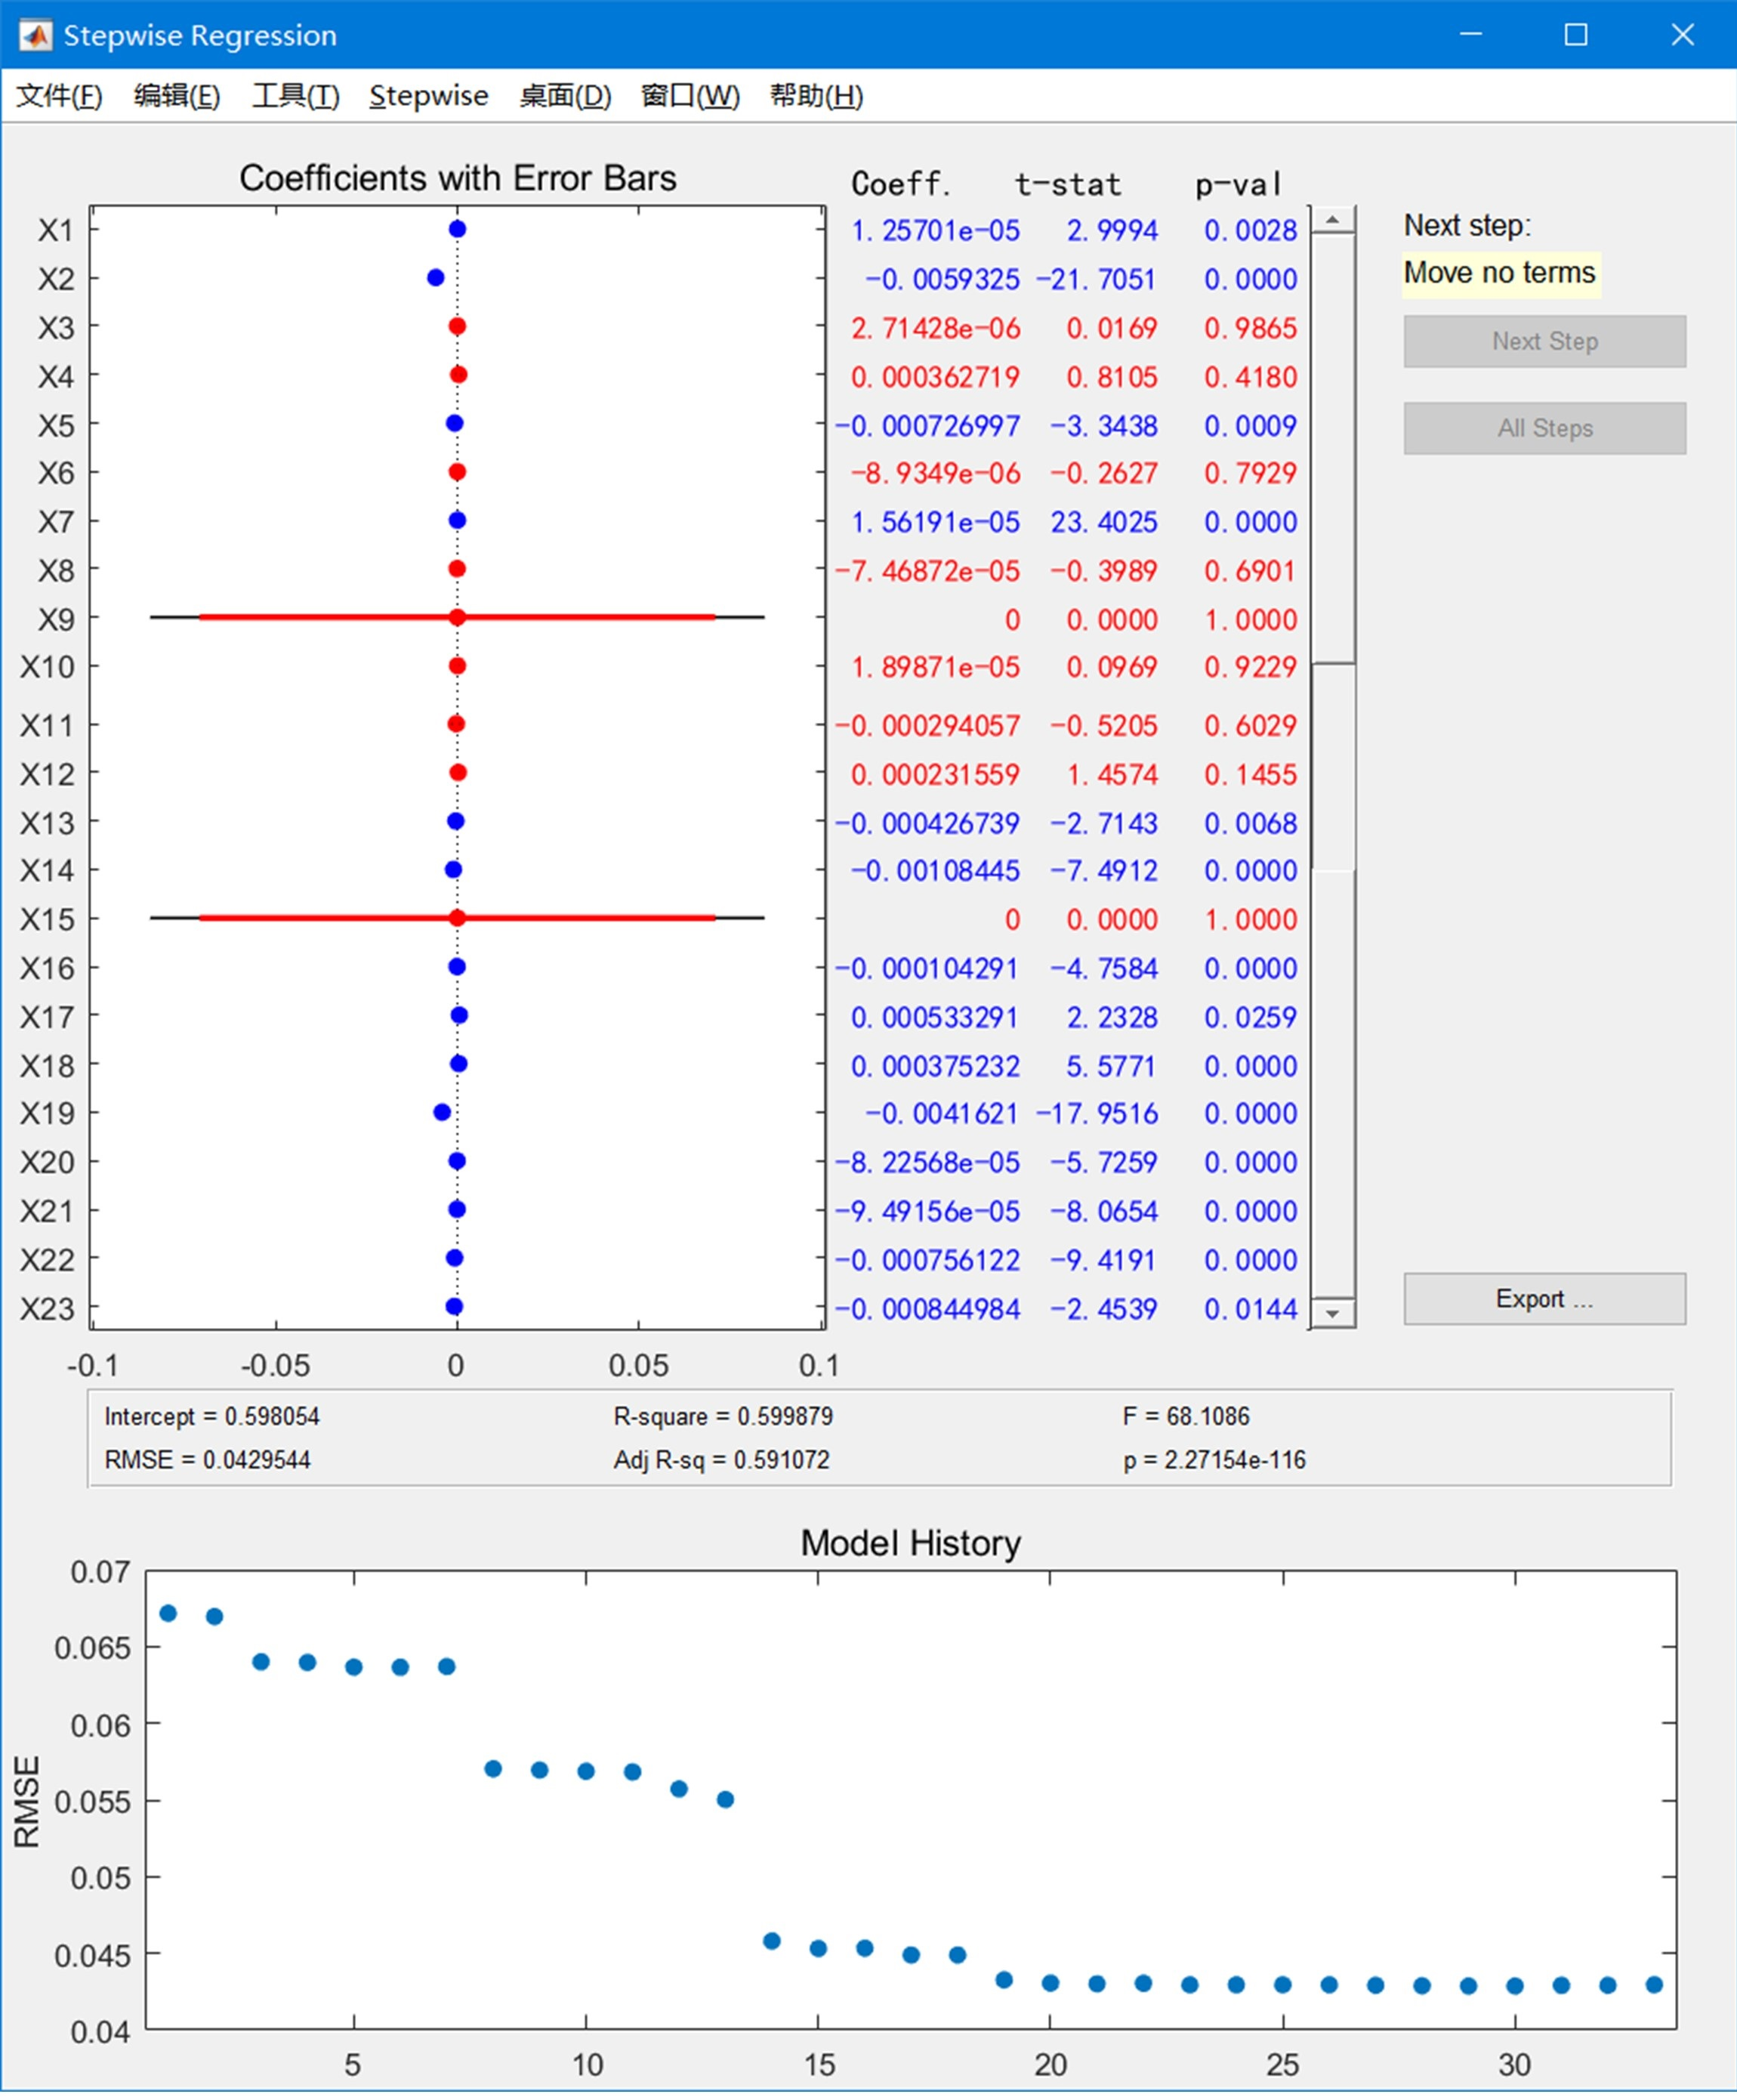
\includegraphics[width=0.5\textwidth]{picture/PPT3} & 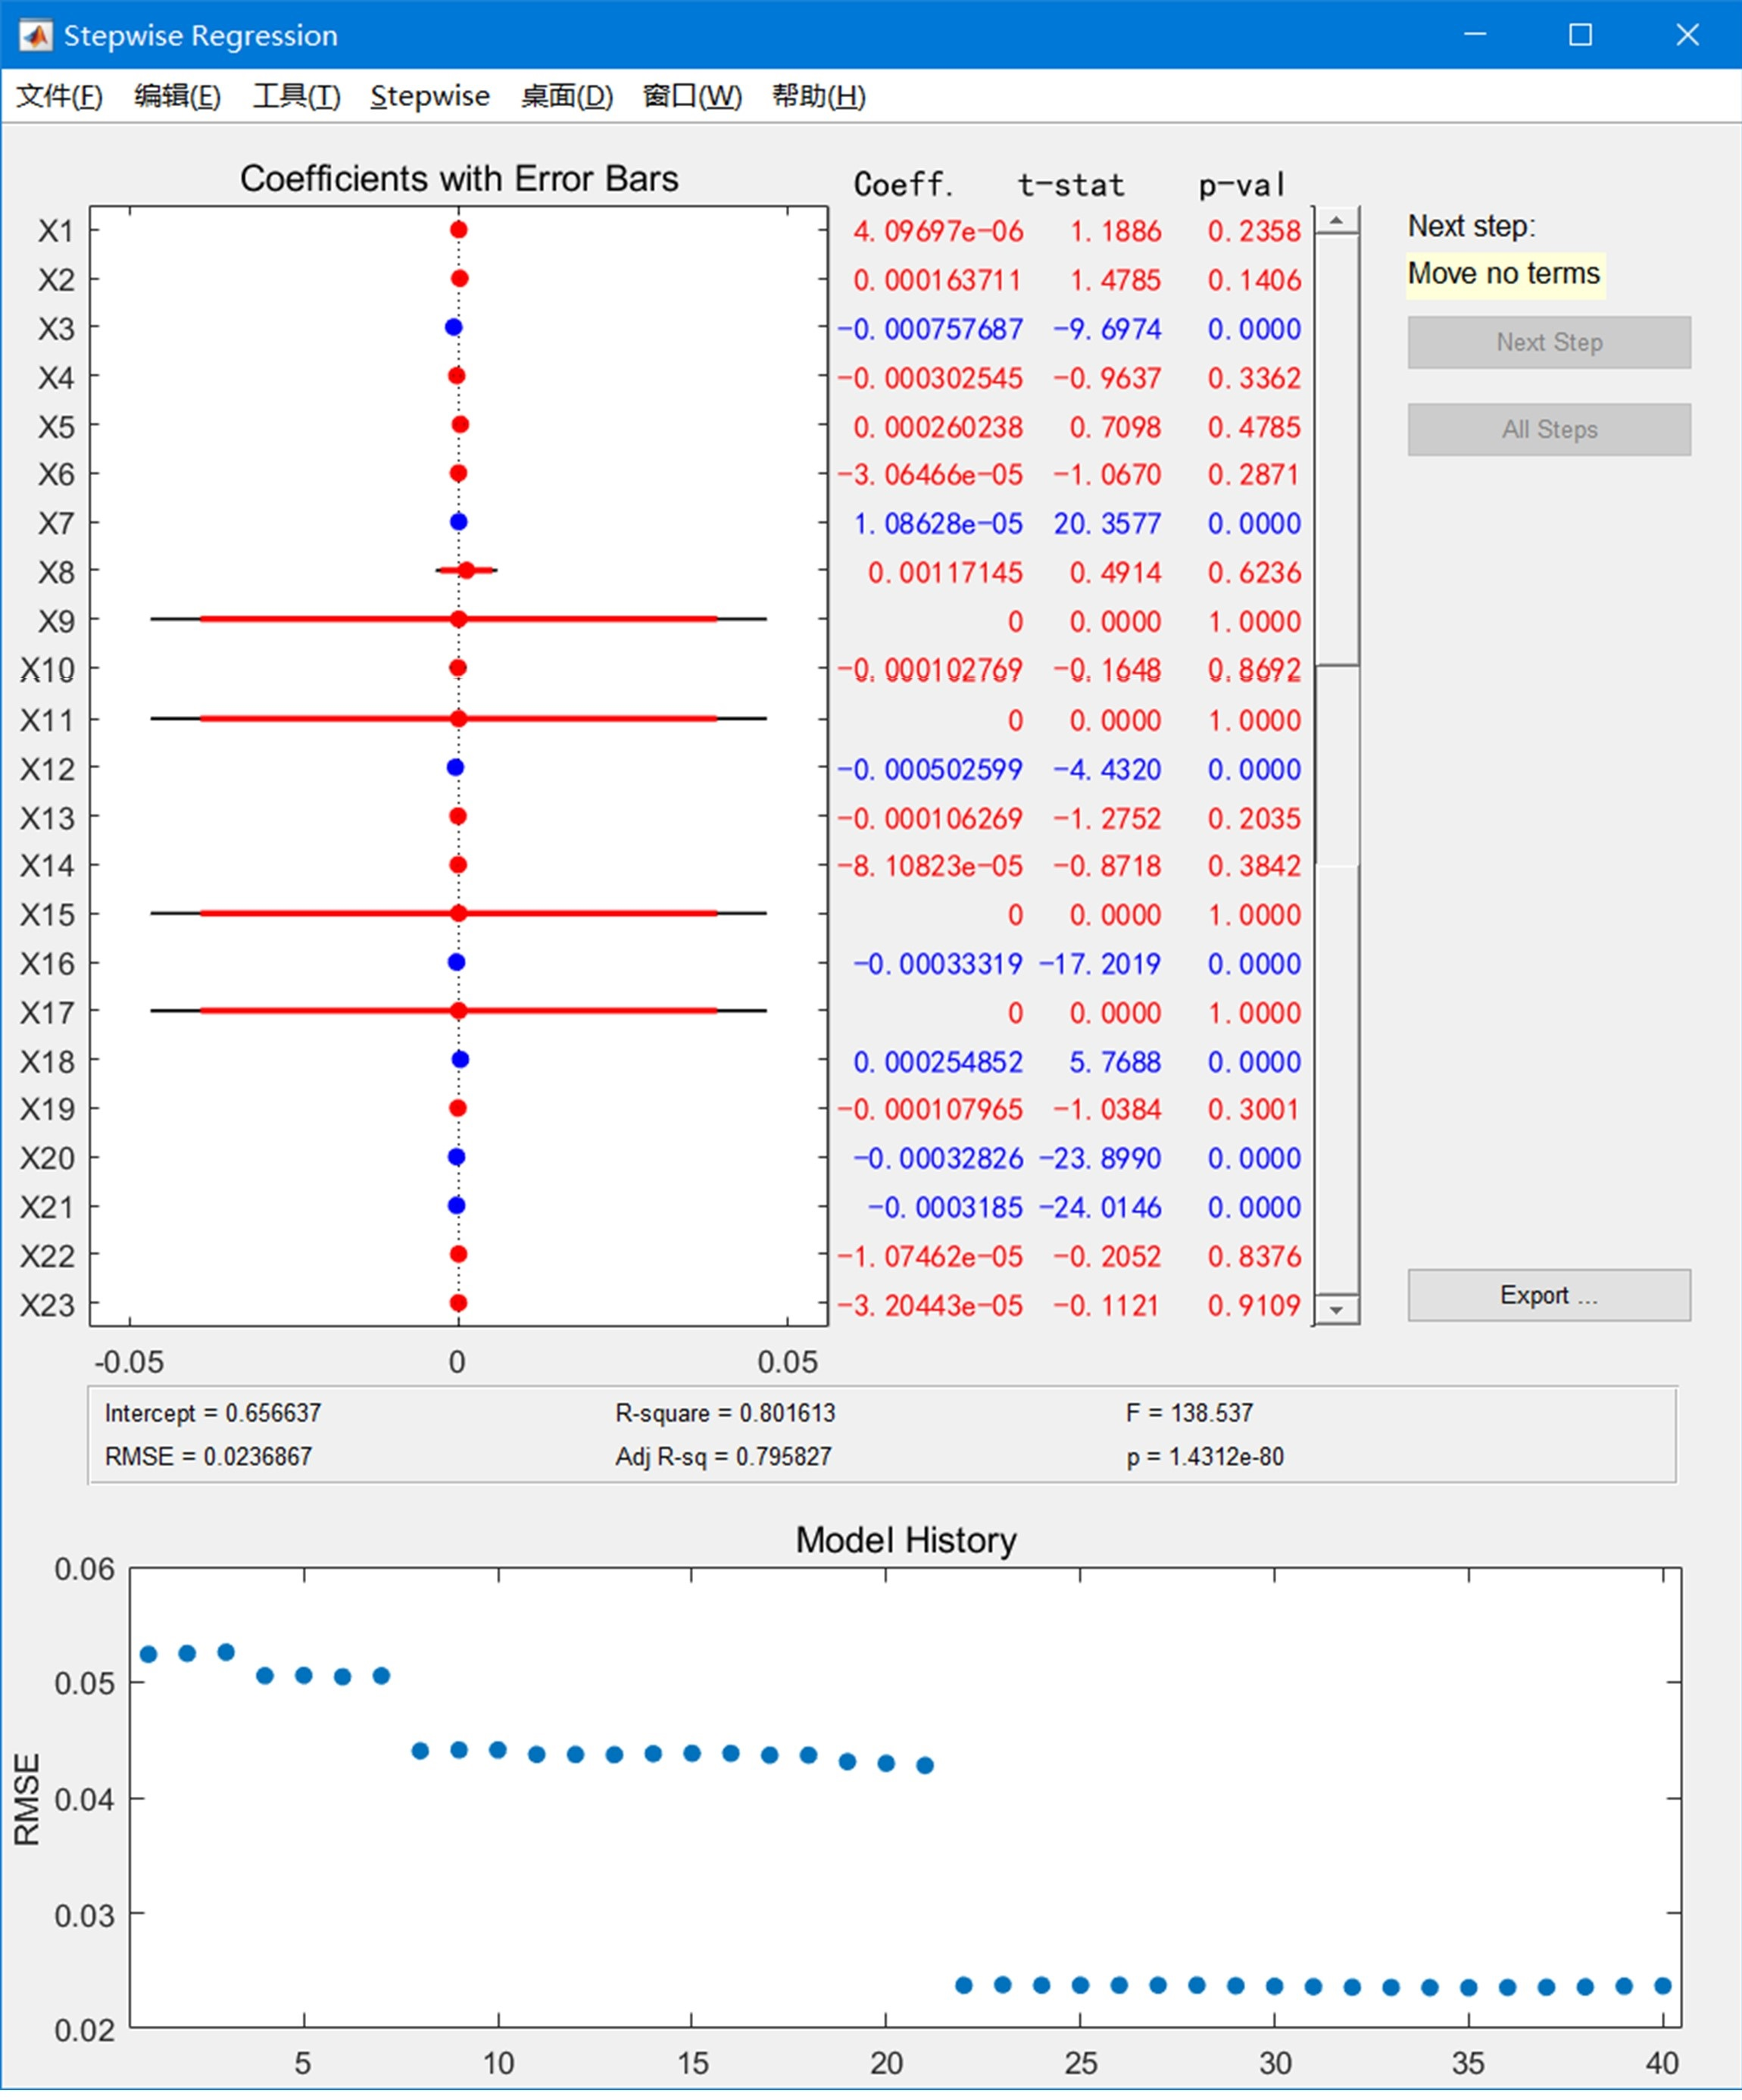
\includegraphics[width=0.5\textwidth]{picture/PPT4} \\
    C & Mn \\
  \end{tabular}
  \caption{C、Mn收得率影响因素逐步回归分析结果}\label{zhubuhuiguifenxi}
\end{figure}

\subsection{模型二:基于多项式回归拟合的收得率预测模型}
\subsubsection{模型的建立}
为了在得知影响因素值的情况下预测C、Mn,我们期望得到收得率关于各影响因素的函数关系式以方便预测。根据泰勒公式,可以表示为:
\begin{equation}\label{taile}
\begin{split}
f(x^1,x^2,\ldots,x^n)=f(x^1_k,x^2_k,\ldots,x^n_k)+\sum_{i=1}^n\left(x^i-x^i_k\right)f′_{x^i}\left(x^1_k,x^2_k,\ldots,x^n_k\right)+\\\frac{1}{2!} \sum_{i,j=1}^n \left(x^i-x^i_k \right)\left(x^j-x^j_k\right)f''_{ij} \left(x^1_k,x^2_k,\ldots,x^n_k\right)+o^n
\end{split}
\end{equation}
其中,$o^n$是高阶无穷小项,当展开项足够时,可以认为与原函数一致。\\
考虑到模型的效率,我们优先求解线性的情况,即:
\begin{equation}\label{xianxing}
  f(X_1,X_2,\ldots,X_{23})=\beta_0+\beta_1 X_1+\ldots+\beta_{23}X_{23}
\end{equation}
\subsubsection{模型的求解}
事实上,在模型一的结果(图\ref{zhubuhuiguifenxi})中,逐步回归法也同时给出了各要素的系数情况。我们得到C和Mn的收得率函数关系为
\begin{equation}\label{chemnxianxing}
\begin{array}{c}
 f_C=\beta_{C_0}+\sum_{i=1}^{23} \beta_{C_i}X_i\\
 \\
 f_{Mn}=\beta_{Mn_0}+\sum_{i=1}^{23} \beta_{Mn_i}X_i\\
 \end{array}
\end{equation}\\
利用得到的收得率函数,分别预测C和Mn的收得率,结果如图\ref{fig:Cyuce}
及图\ref{fig:Mnyuce}
所示。从中可以看出,利用线性回归预测的值比较准确,误差在可接受范围内。
\begin{figure}[htbp]
  \centering
  \begin{tabular}{cc}
  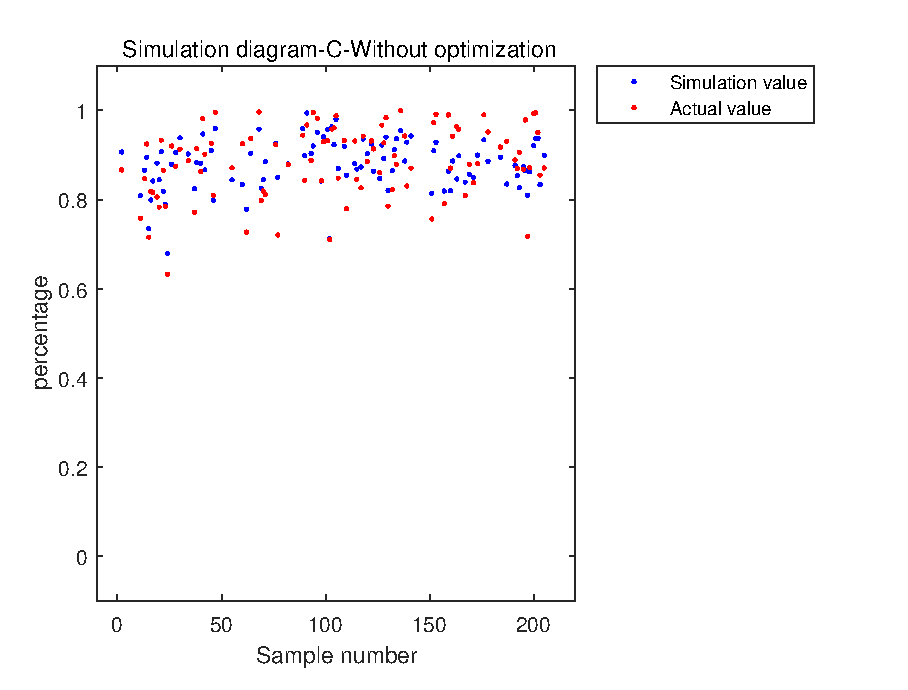
\includegraphics[width=0.5\textwidth]{picture/C_wuxiangduiwucha} & 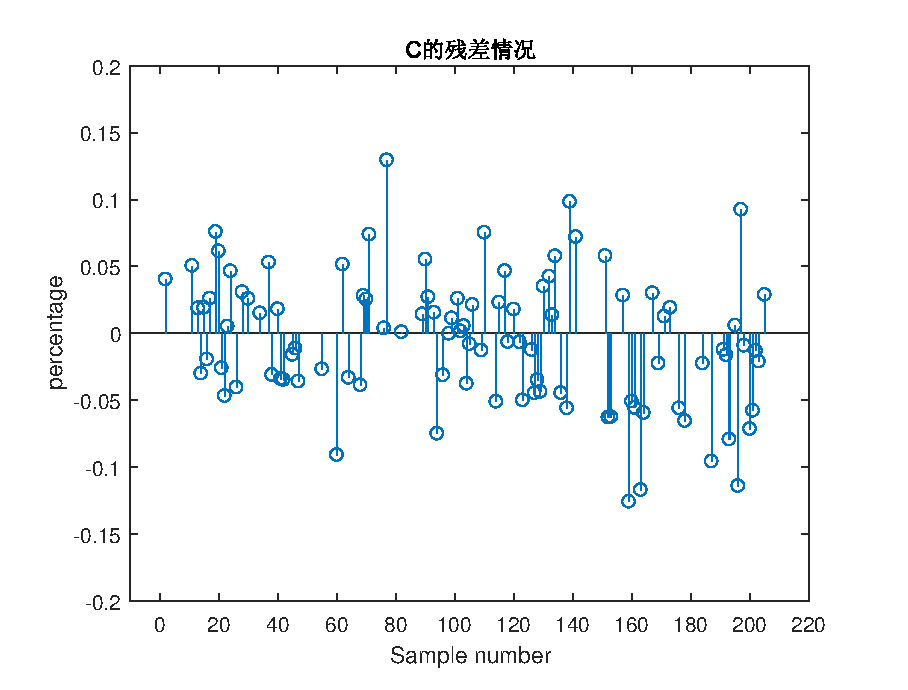
\includegraphics[width=0.5\textwidth]{picture/C_cancha} \\
    C收得率预测 & 残差 \\
  \end{tabular}
  \caption{C收得率预测结果}\label{fig:Cyuce}
\end{figure}
\begin{figure}[htbp]
  \centering
  \begin{tabular}{cc}
  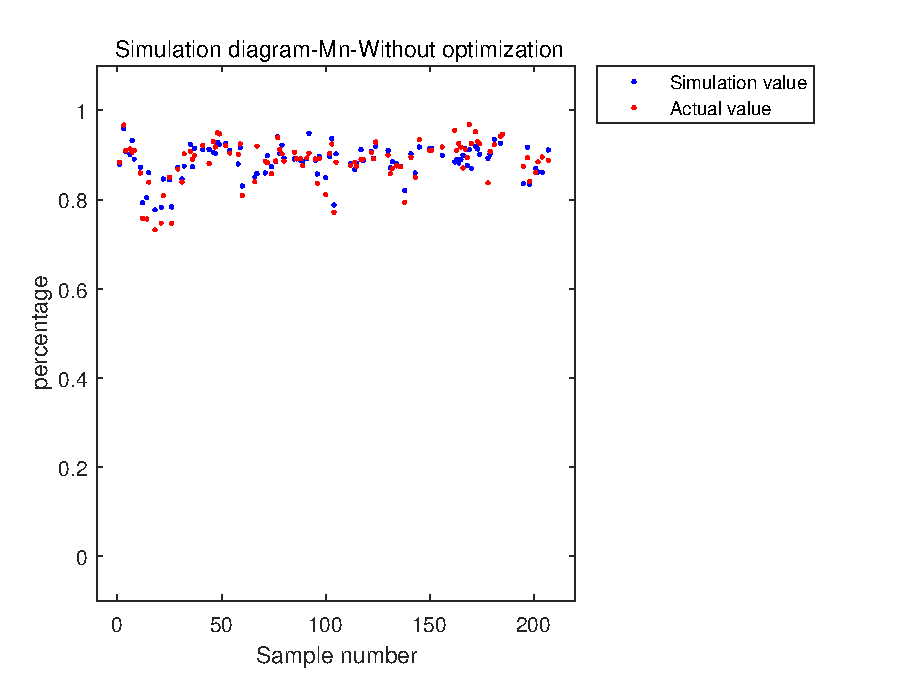
\includegraphics[width=0.5\textwidth]{picture/Mn_wuxiangduiwucha} & 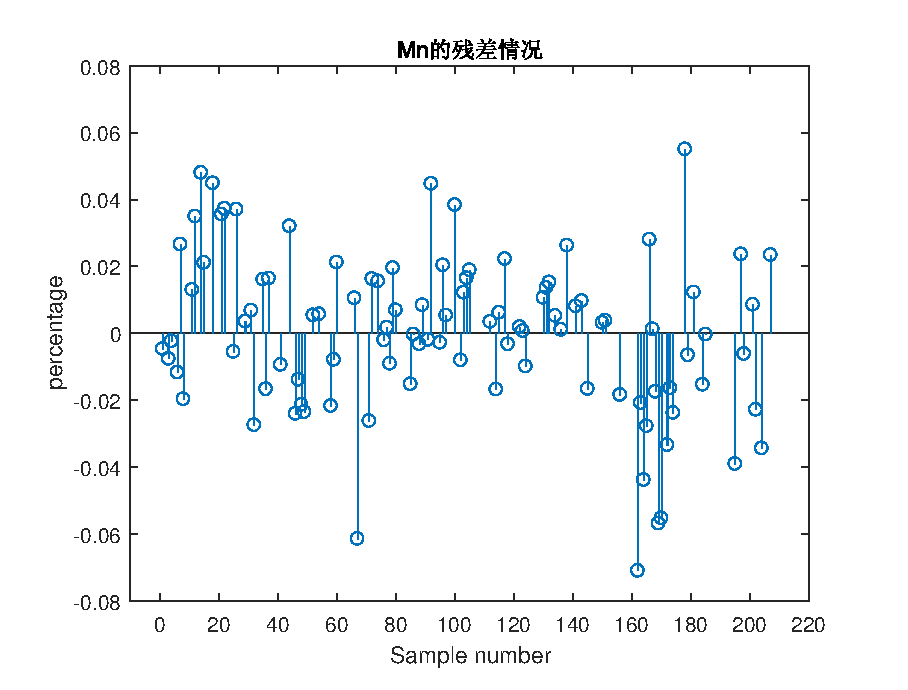
\includegraphics[width=0.5\textwidth]{picture/Mn_cancha} \\
    Mn收得率预测 & 残差 \\
  \end{tabular}
  \caption{Mn收得率预测结果}\label{fig:Mnyuce}
\end{figure}
\subsubsection{考虑高次项实现的模型优化}
利用线性回归得到的预测值误差已经比较小,为了优化模型,考虑高次项的非线性情况。这里以最高次为二次的情况为例,即认为:
\begin{equation}\label{erci}
  f(X_1,X_2,\ldots,X_{23})=\beta_0+\beta_1 X_1+\ldots+\beta_{23}X_{23}+\beta_{24} X_1^2+\beta_{25}X_2^2+\ldots+\beta_{46}X_{23}^2
\end{equation}
同样借助MATLAB工具箱中的STEPWISE,可得到系数情况如图\ref{fig:ercix}
所示。\\
\begin{figure}[htbp]
  \centering
  \begin{tabular}{cc}
  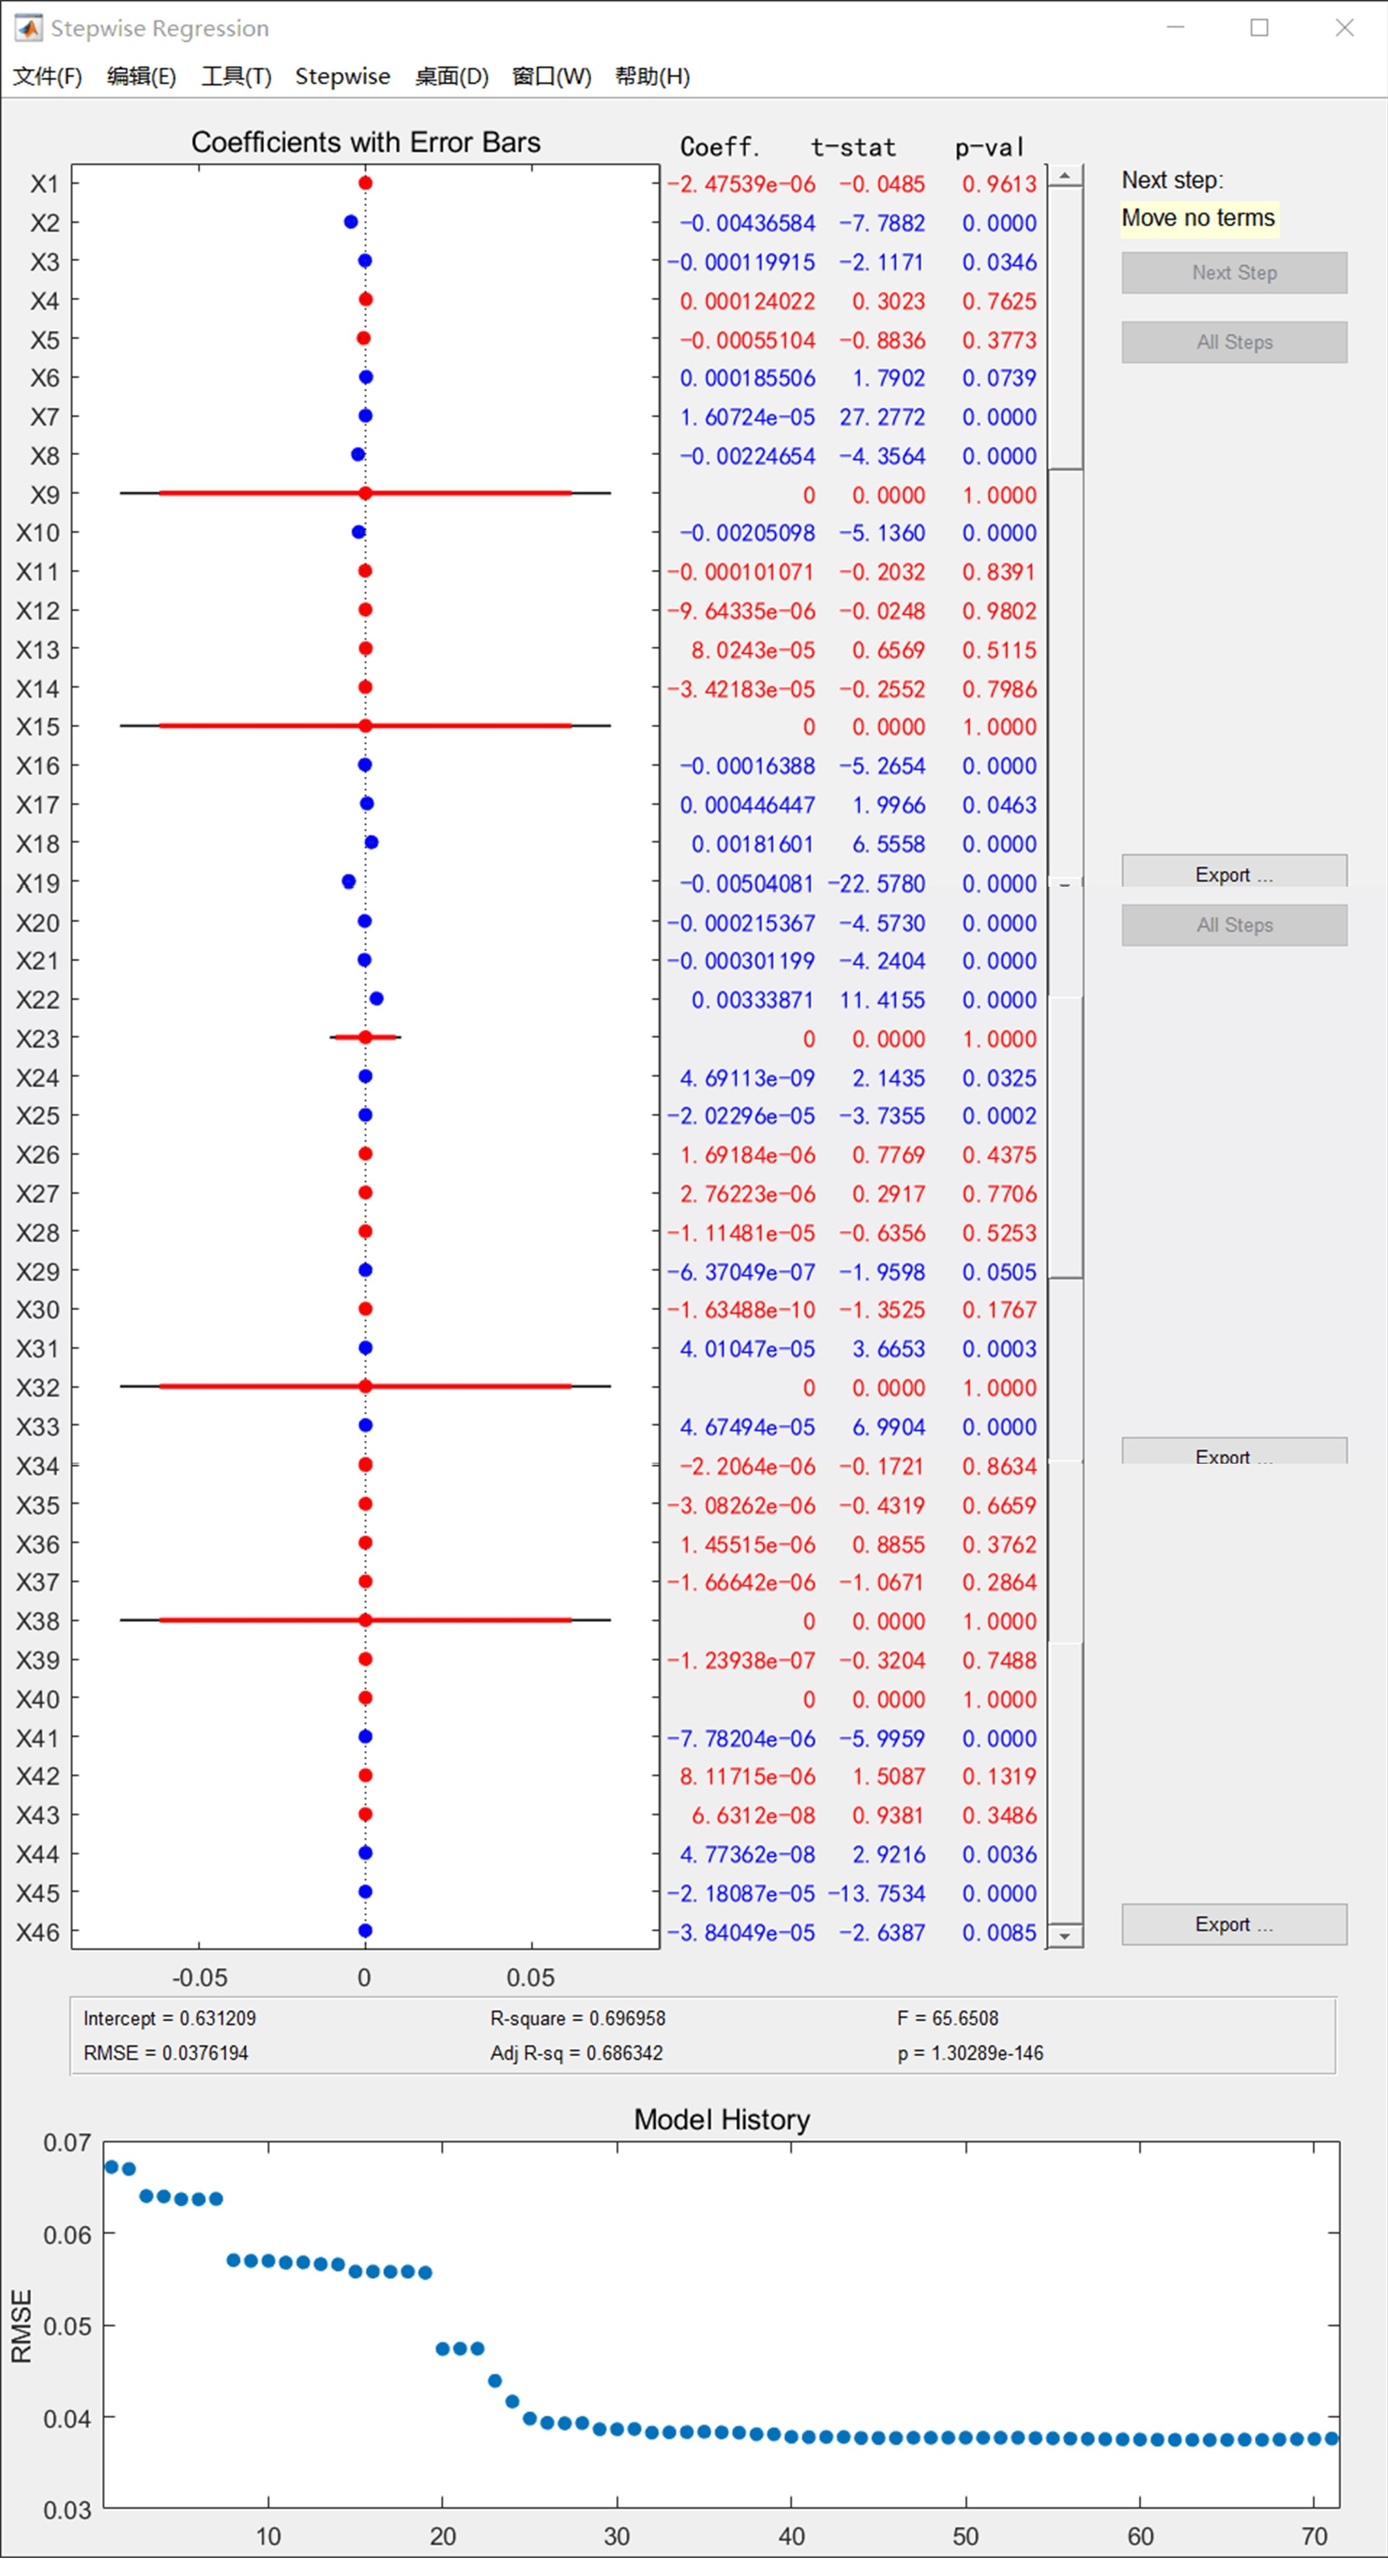
\includegraphics[width=0.5\textwidth]{picture/PPTT1} & 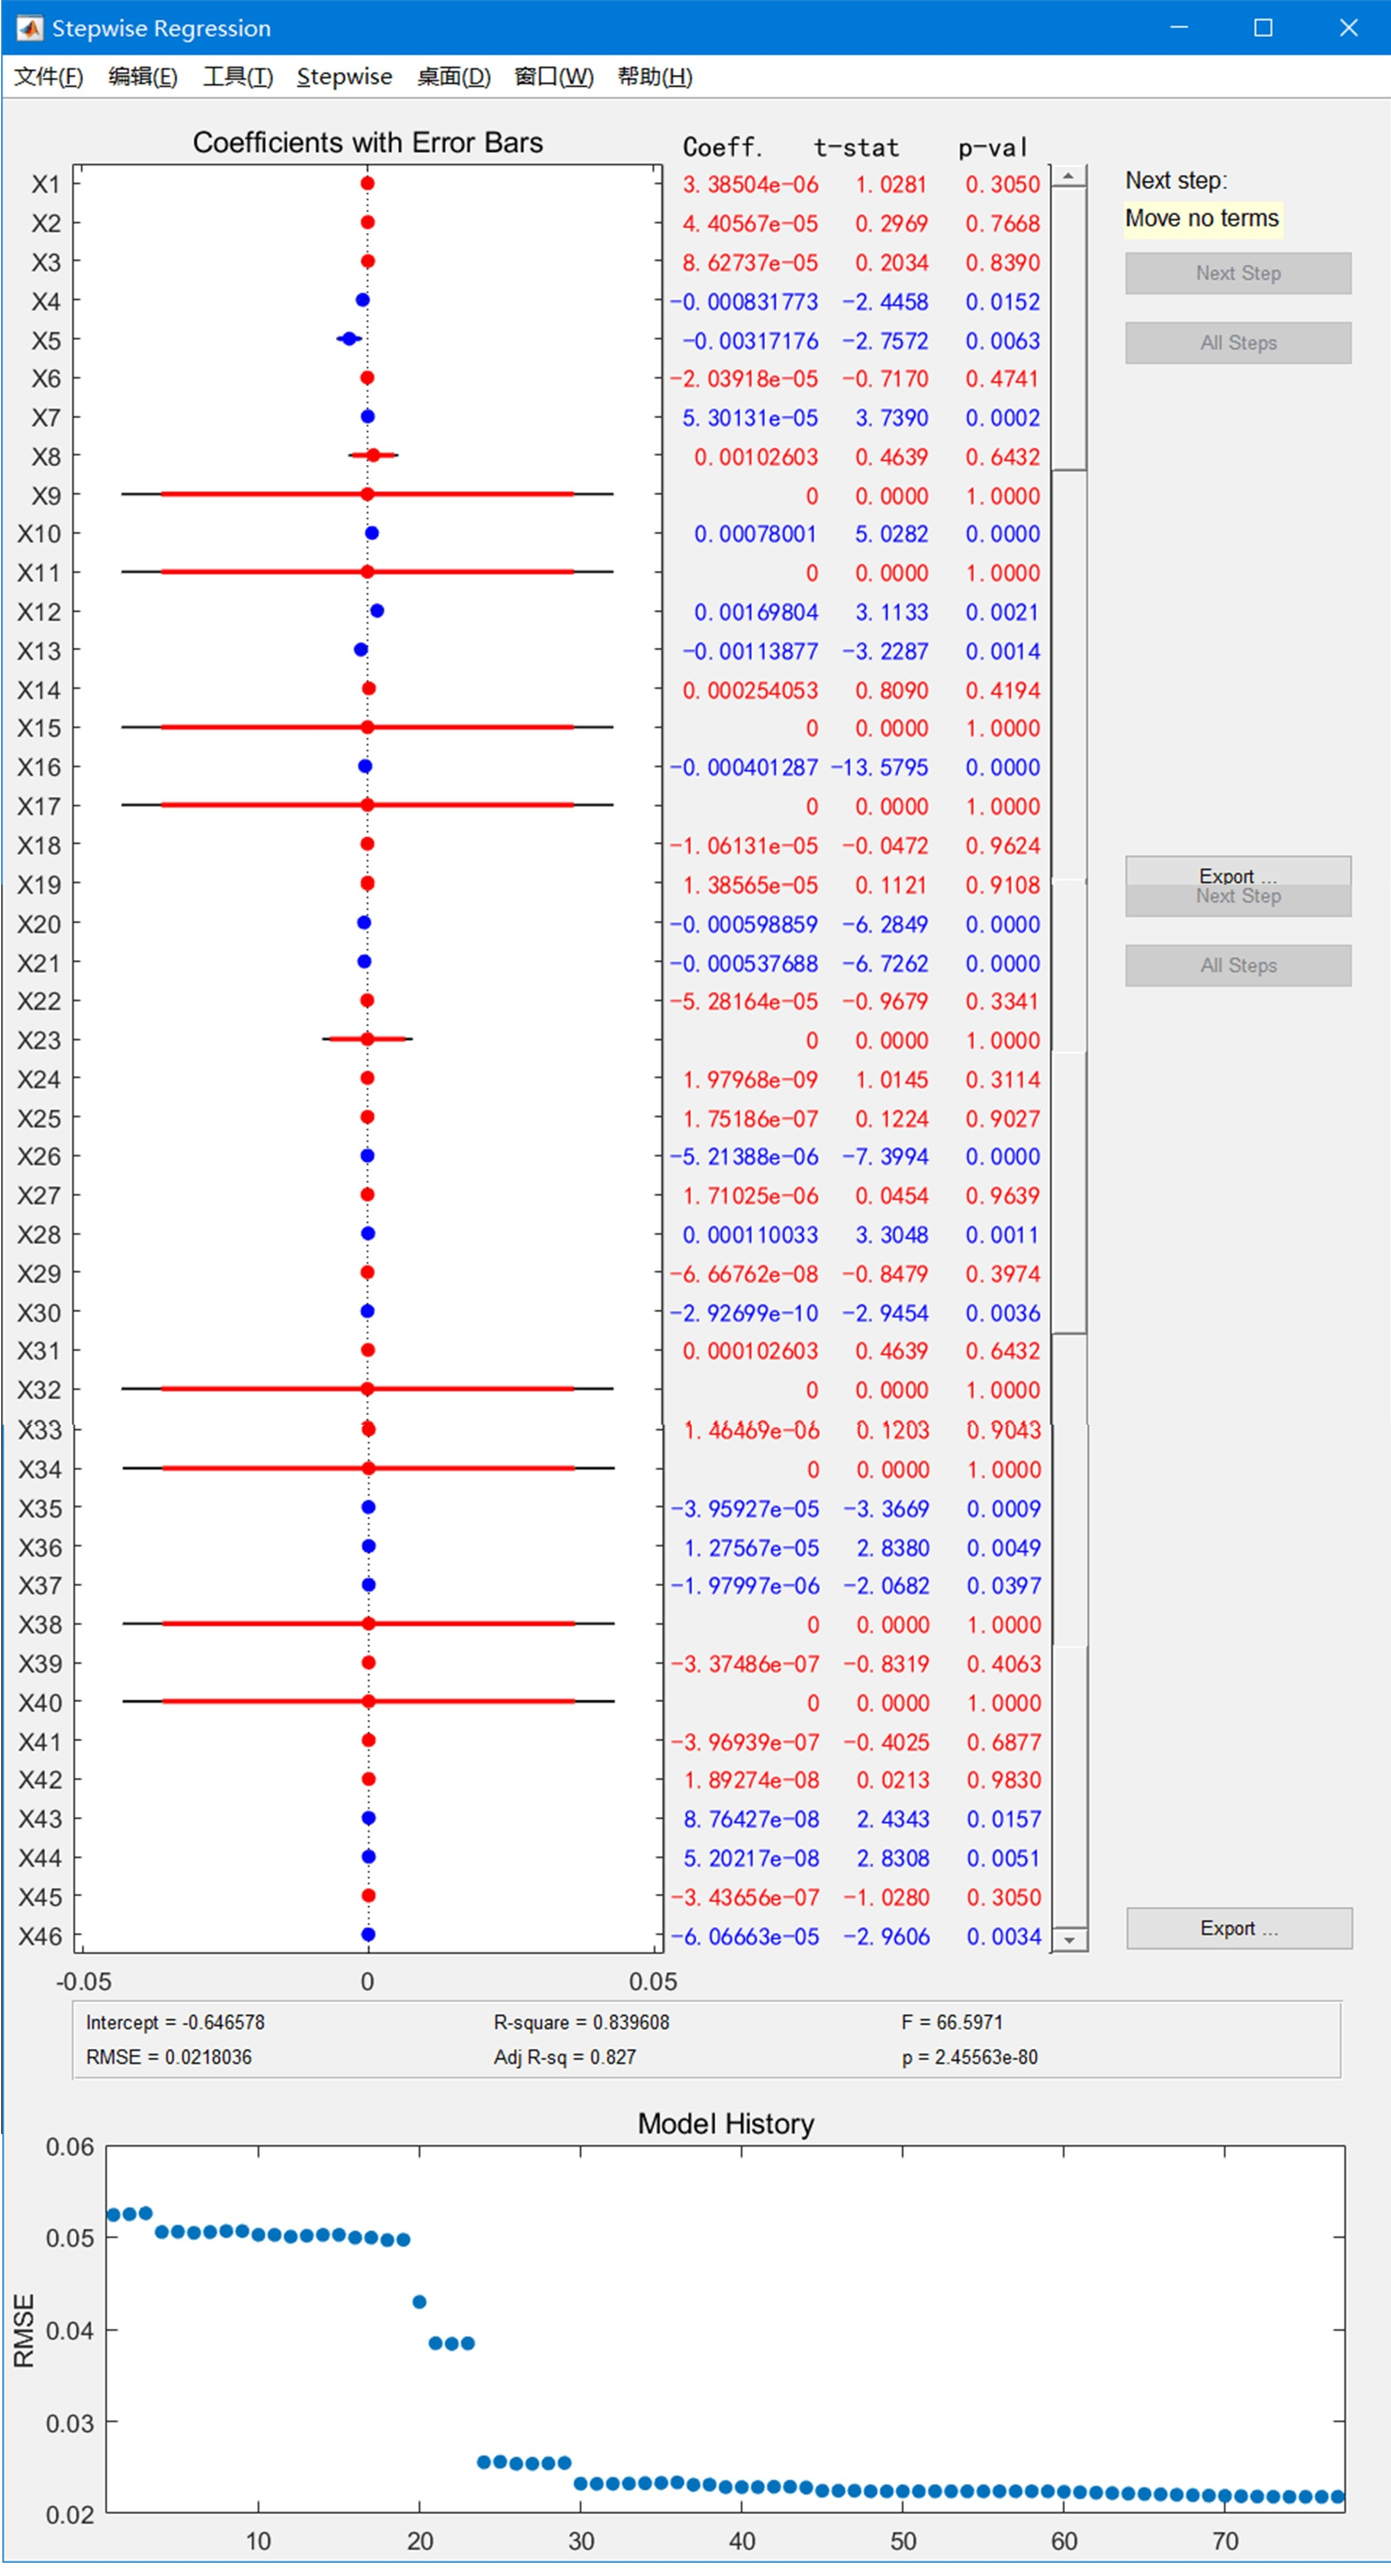
\includegraphics[width=0.5\textwidth]{picture/PPTT2} \\
    C收得率预测系数 & Mn收得率预测系数 \\
  \end{tabular}
  \caption{C,Mn收得率系数-二次项回归时}\label{fig:ercix}
\end{figure}
同样将得到的二次项回归函数预测C和Mn的收得率,并与线性回归函数比较,情况如图\ref{fig:Cyouhua},图\ref{fig:Mnyouhua},表\ref{tab:gaibian}
所示。可知,C、Mn的预测误差分别下降了22.505\%和16.592\%。
\begin{figure}[htbp]
  \centering
  \begin{tabular}{cc}
   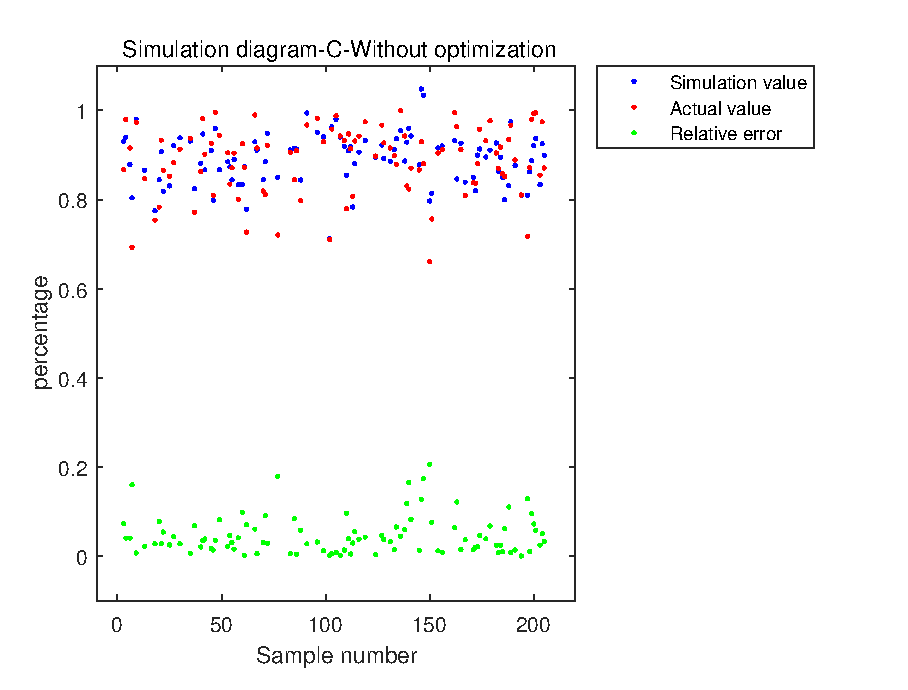
\includegraphics[width=0.5\textwidth]{picture/C1}  &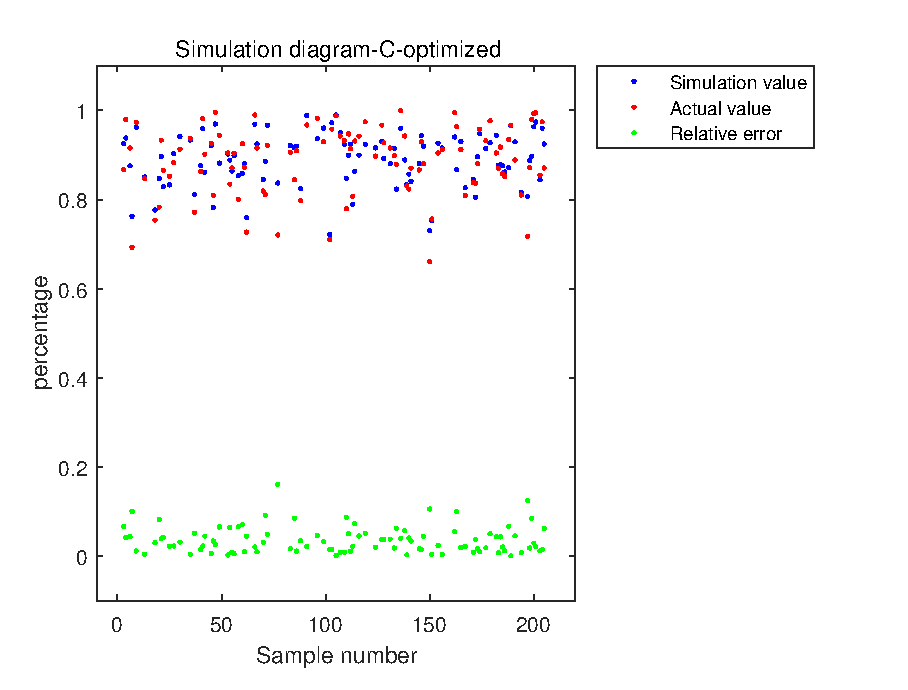
\includegraphics[width=0.5\textwidth]{picture/C2}   \\
    C收得率预测-优化前  &  C收得率预测-优化后 \\
    \multicolumn{2}{c}{ 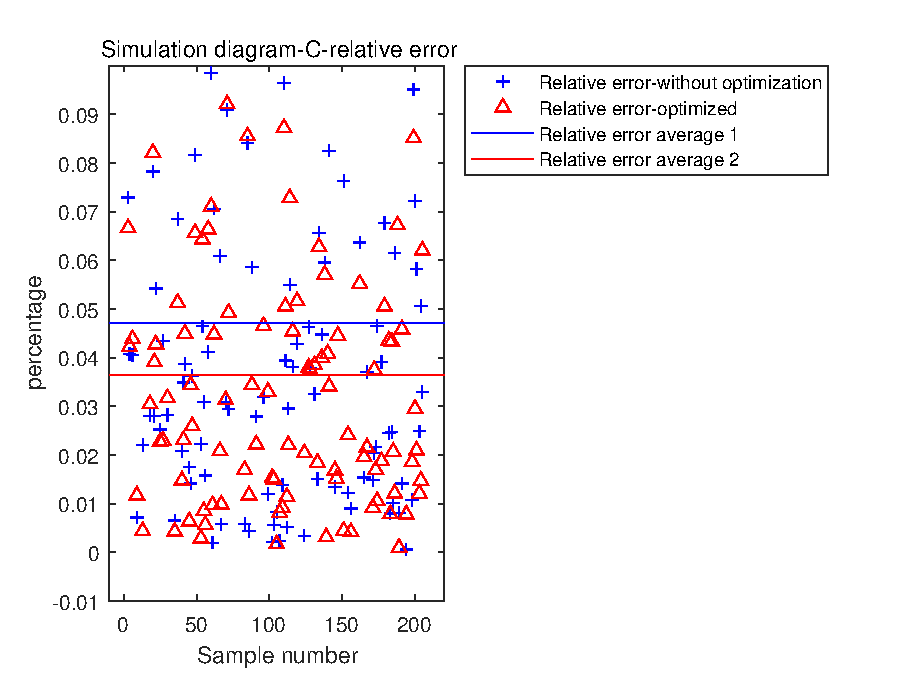
\includegraphics[width=0.5\textwidth]{picture/C3}}   \\
     \multicolumn{2}{c}{相对误差}   \\
  \end{tabular}
  \caption{优化前后C收得率预测情况}\label{fig:Cyouhua}
\end{figure}
\begin{figure}[htbp]
  \centering
  \begin{tabular}{cc}
   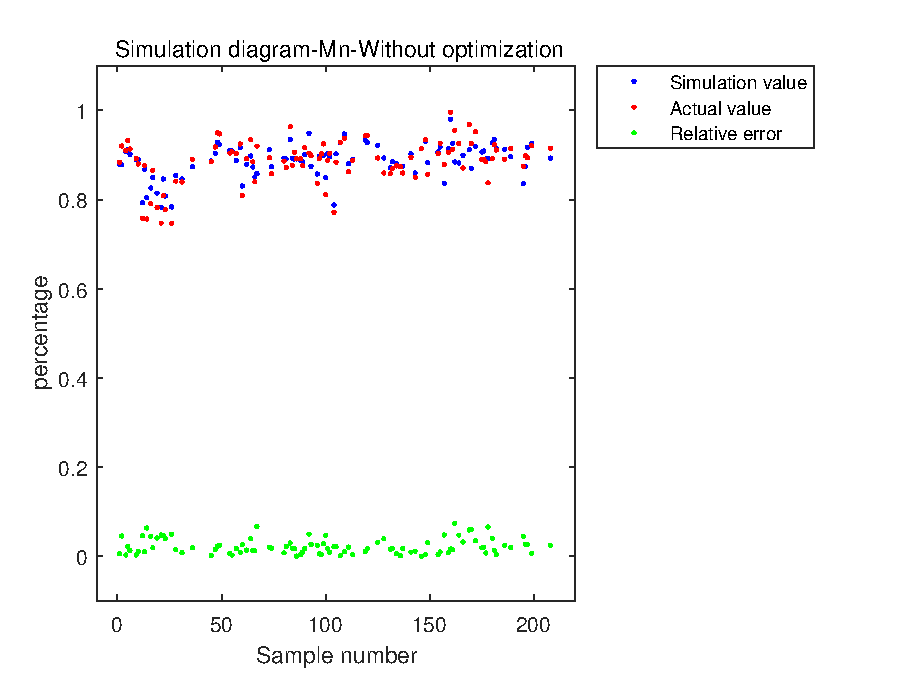
\includegraphics[width=0.5\textwidth]{picture/Mn1}  &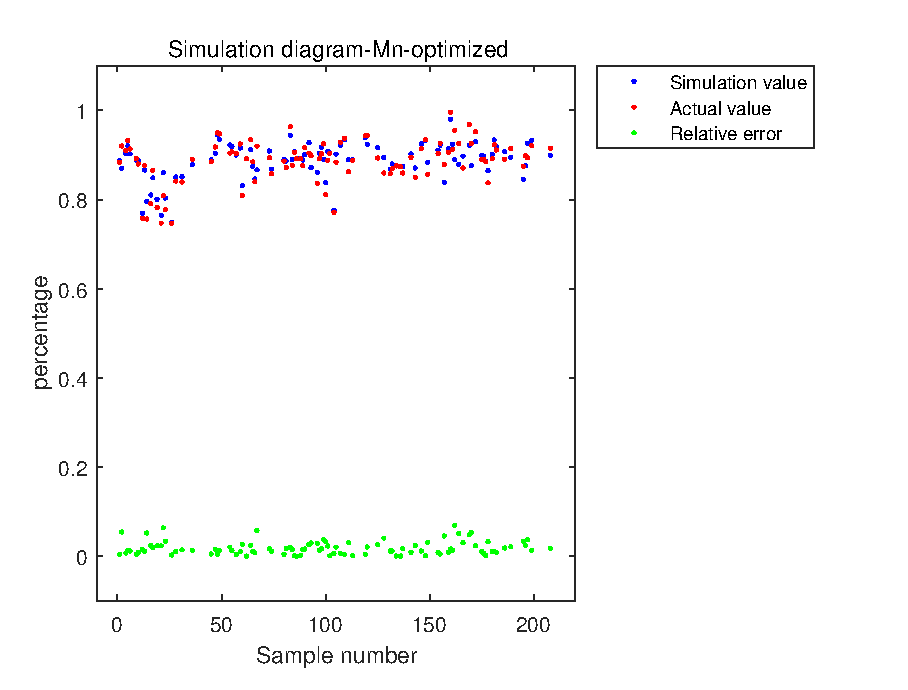
\includegraphics[width=0.5\textwidth]{picture/Mn2}   \\
    Mn收得率预测-优化前  &  Mn收得率预测-优化后 \\
    \multicolumn{2}{c}{ 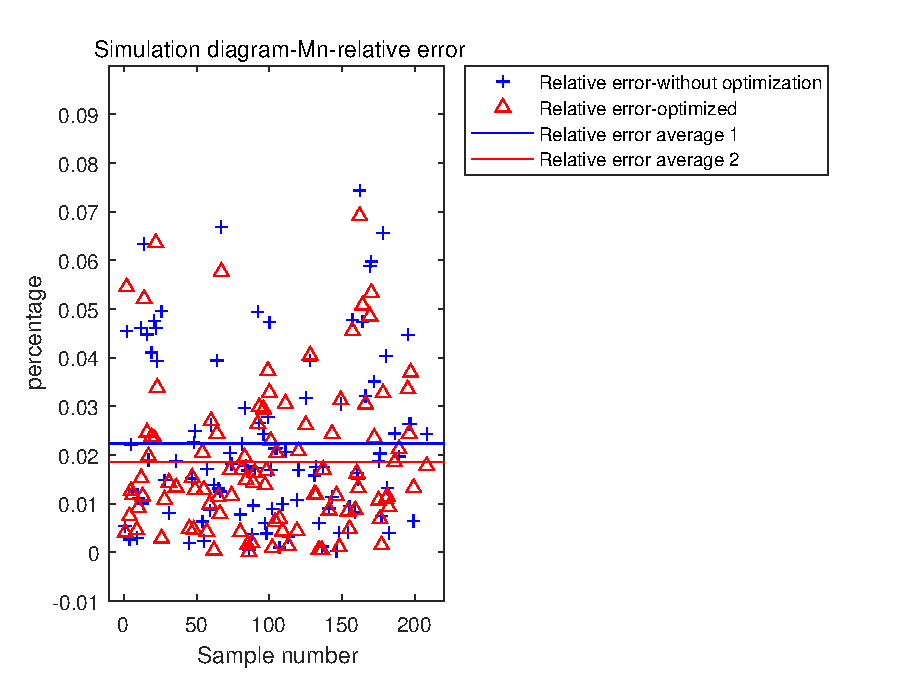
\includegraphics[width=0.5\textwidth]{picture/Mn3}}   \\
     \multicolumn{2}{c}{相对误差}   \\
  \end{tabular}
  \caption{优化前后Mn收得率预测情况}\label{fig:Mnyouhua}
\end{figure}

\begin{table}[htbp]
  \centering
  \caption{优化前后收得率预测相对误差均值}
    \begin{tabular}{ccc}
    \hline
      & C & Mn \\
      \hline
    优化前相对误差均值 & 4.710\% & 2.230\% \\
    优化后相对误差均值 & 3.650\% & 1.860\% \\
    下降率 & 22.505\% & 16.592\% \\
    \hline
    \end{tabular}%
  \label{tab:gaibian}%
\end{table}%

\subsection{模型三:基于约束优化算法的成本优化模型}
重复模型二中的过程,得到(其中S元素由于源数据精度不够,无法拟合得到显式的表达式)其余元素的收得率情况。其中,系数计算见图\ref{fig:ercixP}
。
\begin{figure}[htbp]
  \centering
  \begin{tabular}{cc}
  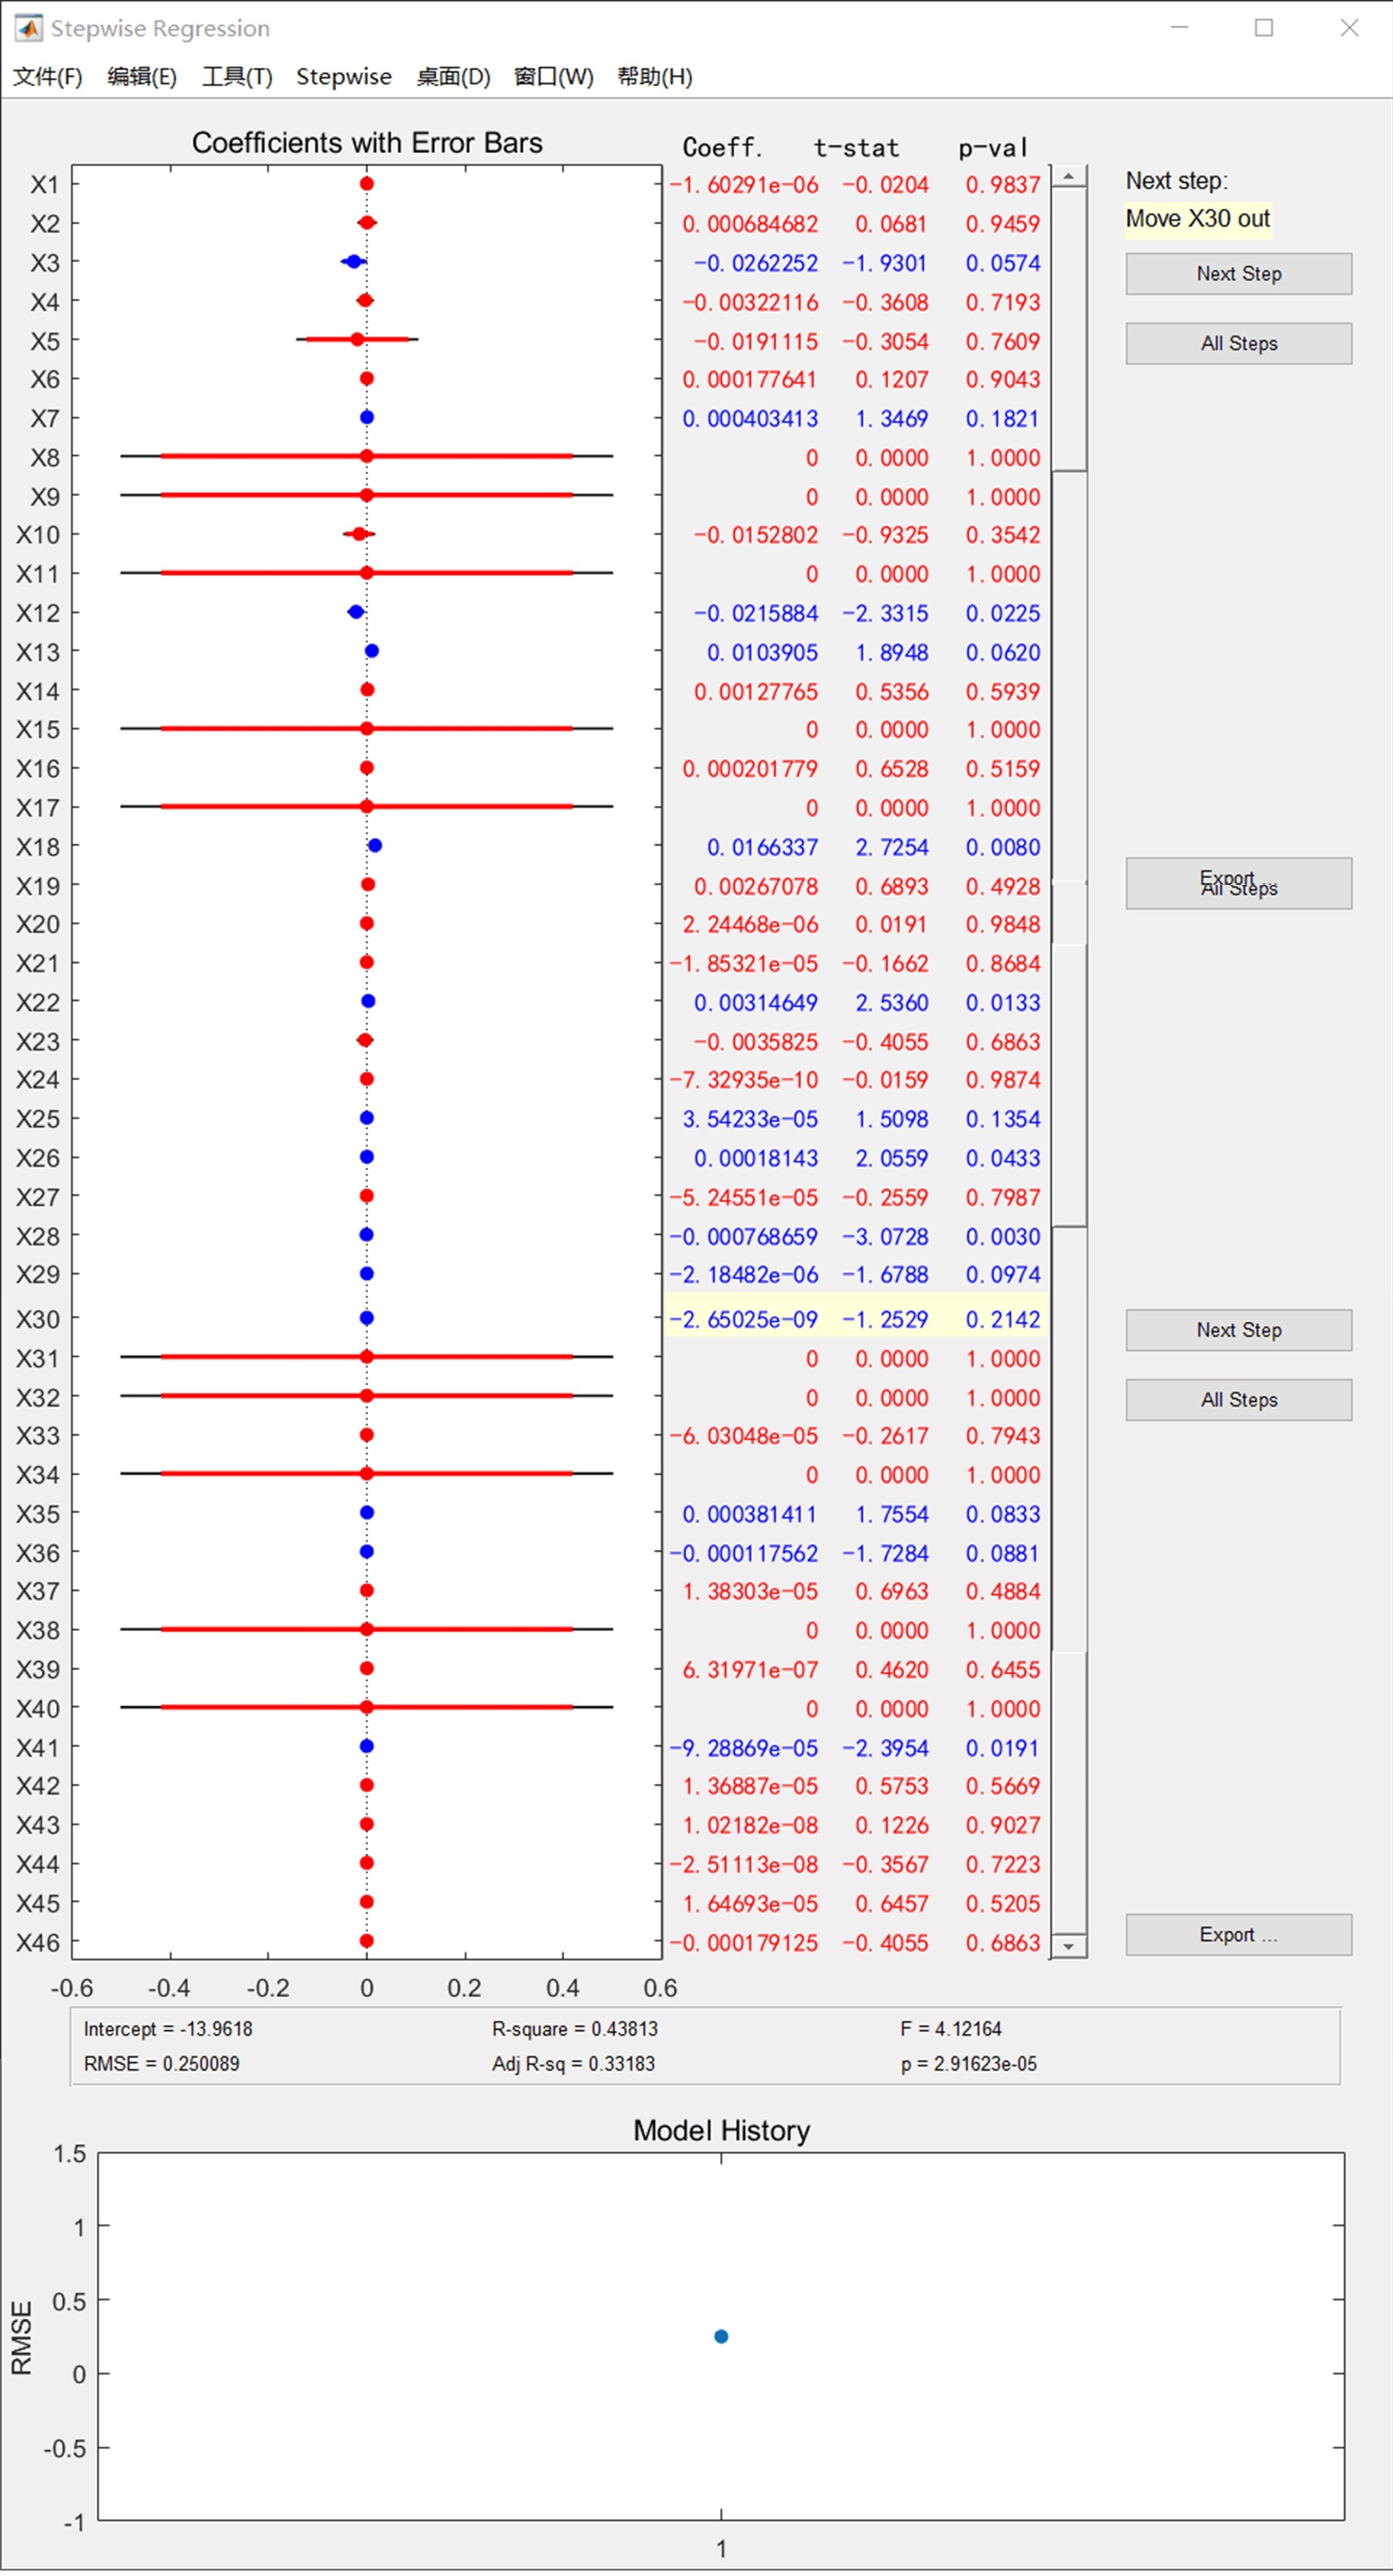
\includegraphics[width=0.5\textwidth]{picture/PPTT3} & 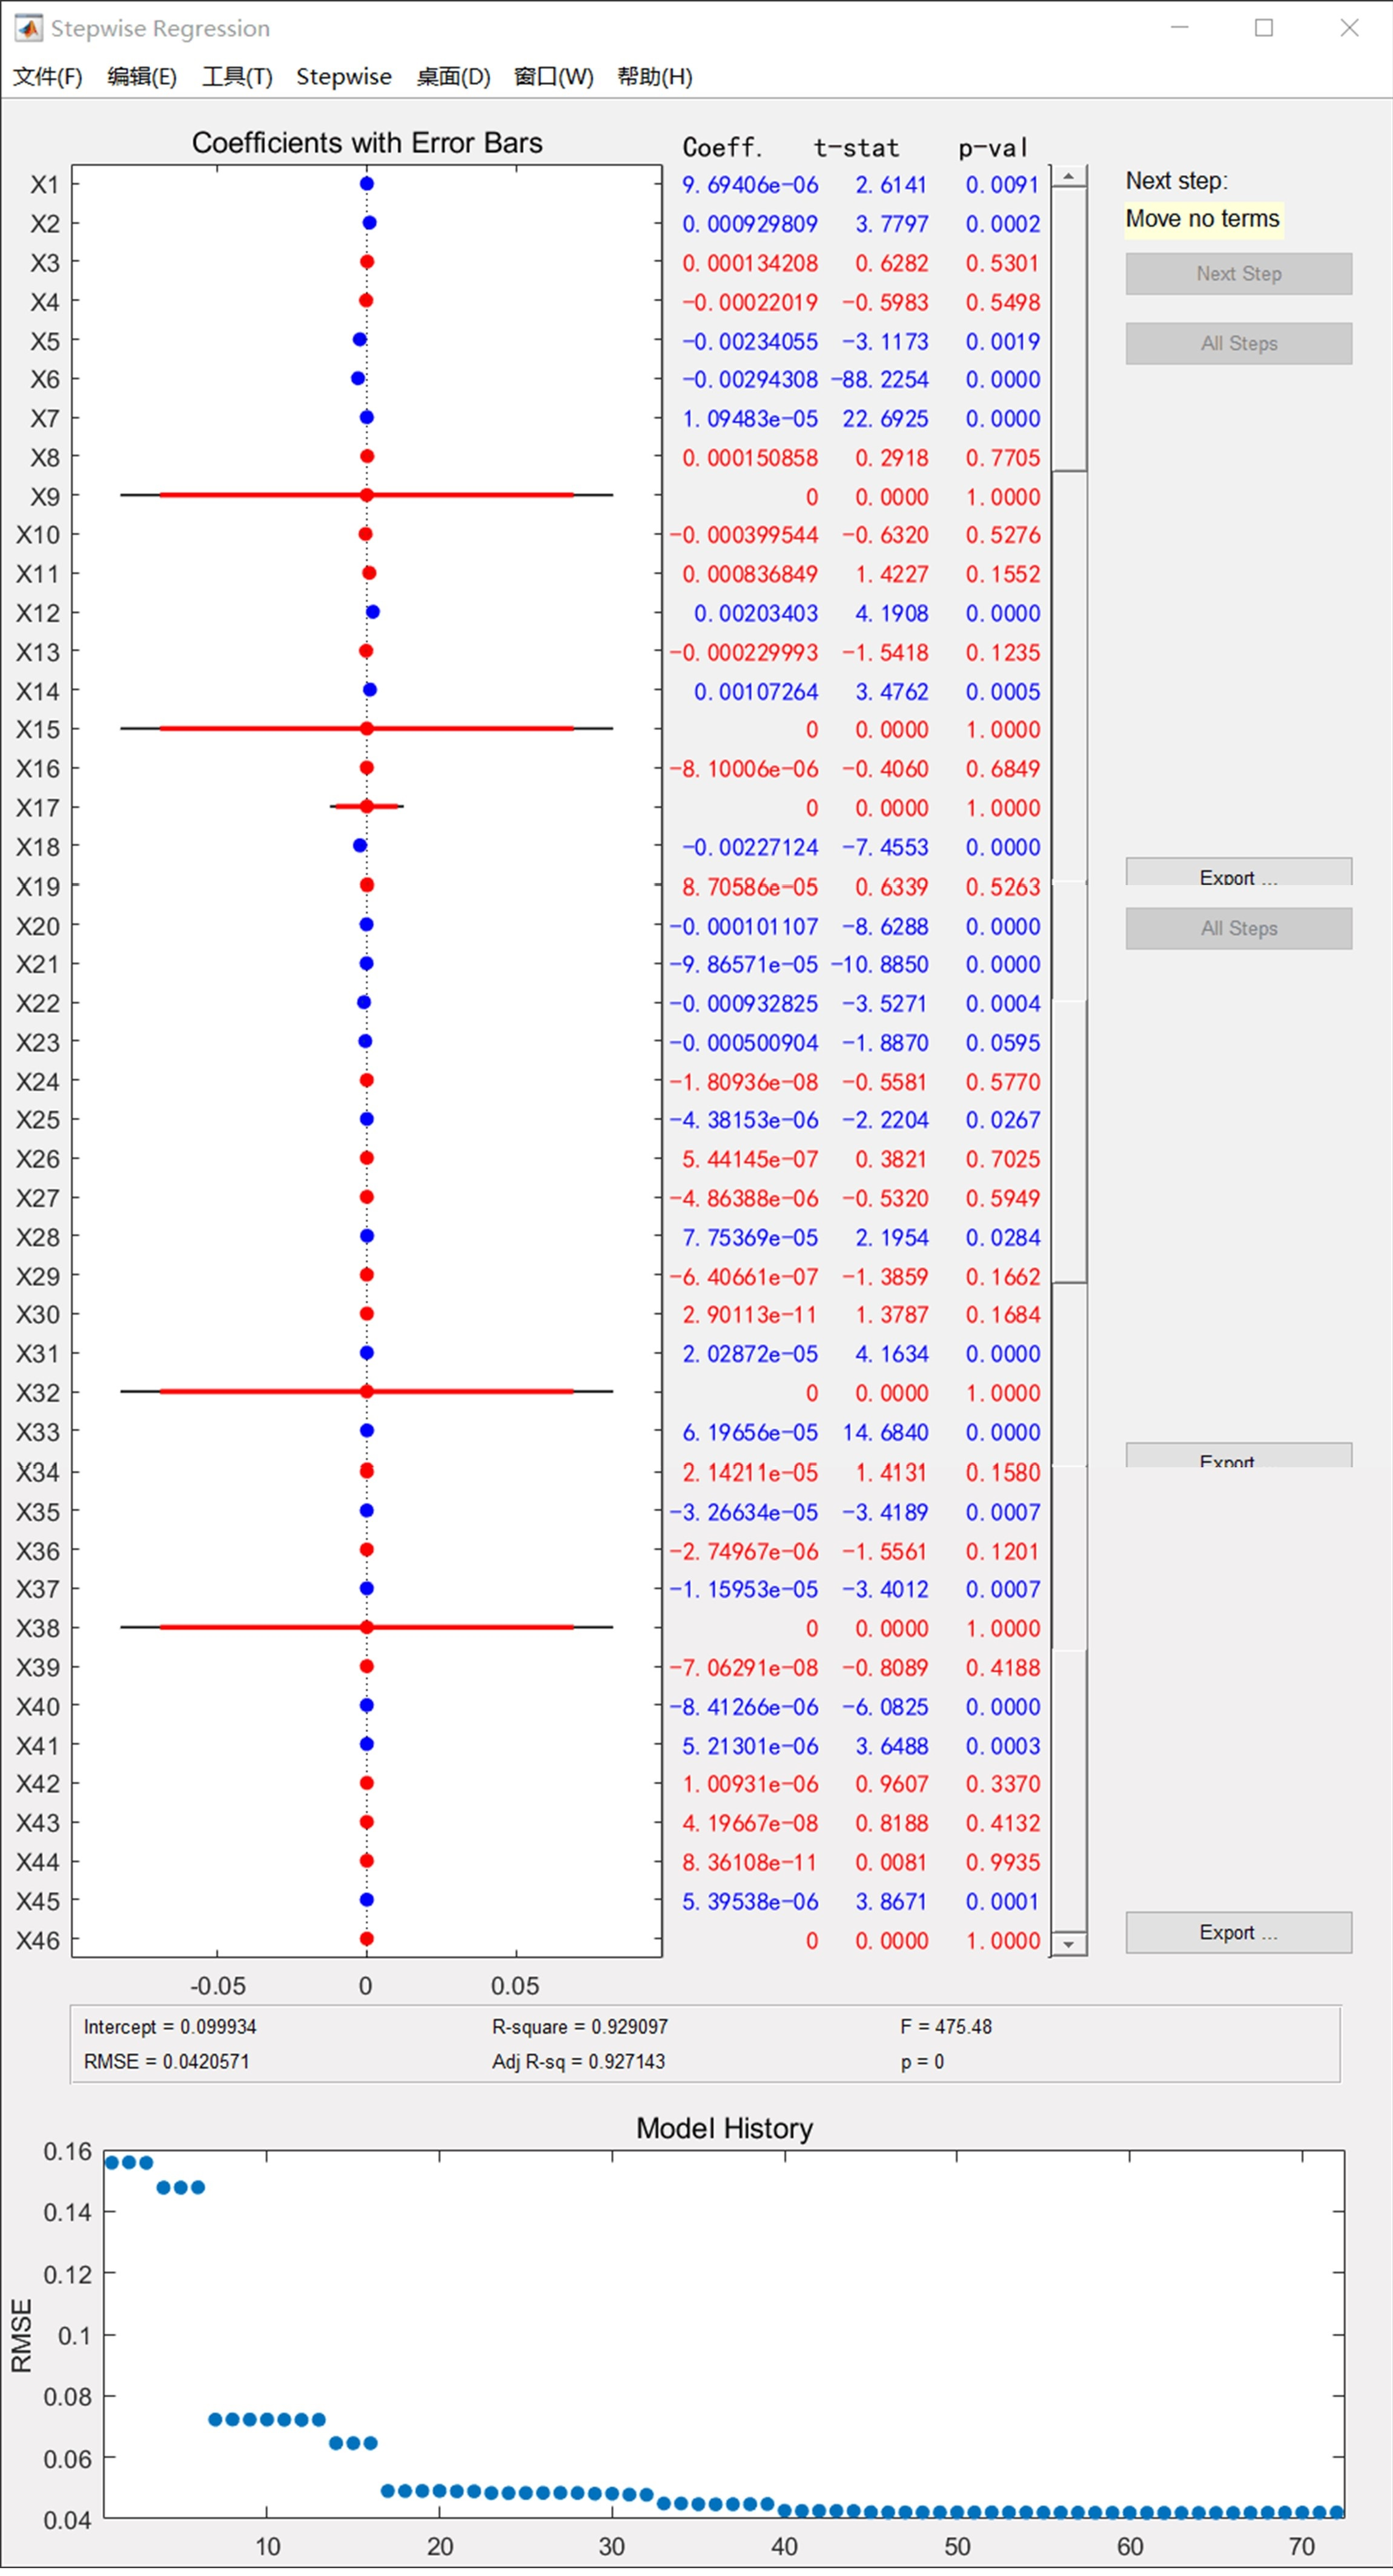
\includegraphics[width=0.5\textwidth]{picture/PPTT4} \\
    P收得率预测系数 & Si收得率预测系数 \\
  \end{tabular}
  \caption{P,Si收得率系数-二次项回归时}\label{fig:ercixP}
\end{figure}
将目标值、收得率作为约束条件,计算成本的最小值。
\subsubsection{模型的建立}
所求目标为:
\begin{equation}\label{mubiao1}
\min \sum_{i=8}^{23}X_i\cdot PRICE_{i}
\end{equation}
约束条件为:
\begin{equation}\label{zhuanhualv2333re}
\left\{
             \begin{array}{cc}
0.19\% X_7 \leq f_C\sum_{i=8}^{23}X_iMC_i+X_2 \leq 0.25\% X_7\\
1.30\% X_7 \leq f_{Mn}\sum_{i=8}^{23}X_iMMn_i+X_3 \leq 1.60\% X_7\\
0.50\% X_7 \leq f_{Si}\sum_{i=8}^{23}X_iMSi_i+X_6 \leq 0.60\% X_7\\
  f_{P}\sum_{i=8}^{23}X_iMP_i+X_5 \leq 0.04\% X_7\\
  X_i\geq 0&i=1,2,\ldots,23\\
 \end{array}
\right.
\end{equation}
\subsubsection{模型的求解}
虽然,通过式\ref{zhuanhualv2333re}也有可能求解,但这样效率太低。我们采用拉格朗日乘子法和KKT条件,实现算法的优化。

构建拉格朗日算子
\begin{equation}\label{lagelangr}
  L(x,\alpha,\beta)=f(x)+\sum_{i=1}^{m}\alpha_i h_i(x)+\sum_{j=1}^{n}\beta_i g_i(x)
\end{equation}
其中,$h_(x),g_i(x)$为各种约束条件。求:
\begin{equation}\label{lagelangr2}
 \left\{
             \begin{array}{cc}
             \nabla_x L(x,\alpha,\beta)=0\\
             \beta_jg_j(x)=0&j=1,2,\ldots,n\\
             h_i(x)=0&i=1,2,\ldots,m\\
             g_j\leq 0&j=1,2,\ldots,n\\
             \beta_j\geq 0&j=1,2,\ldots,n\\
              \end{array}
\right.
\end{equation}
这大大简化了约束条件的计算。

用MATLAB求解拉格朗日乘子法和KKT条件下的约束模型,
针对2种炉号的钢材原料情况,我们给出推荐的合金配比方案,见表\ref{tab:tuij}。
\begin{table}[htbp]
  \centering
  \caption{投料推荐表}
    \begin{tabular}{|c|cc|cc|}
    \hline
    炉号 & \multicolumn{2}{c|}{7A06625} & \multicolumn{2}{c|}{7A06620} \\
    \hline
      & 原始投料 & 推荐投料 & 原始投料 & 推荐投料 \\
    氮化钒铁FeV55N11-A & 0 & 13 & 0 & 0 \\
    低铝硅铁 & 0 & 1 & 0 & 332 \\
    钒氮合金(进口) & 78 & 0 & 79 & 0 \\
    钒铁(FeV50-A) & 0 & 0 & 0 & 0 \\
    钒铁(FeV50-B) & 0 & 0 & 0 & 0 \\
    硅铝钙 & 0 & 45 & 0 & 431 \\
    硅铝合金FeAl30Si25 & 50 & 0 & 50 & 54 \\
    硅铝锰合金球 & 0 & 0 & 0 & 0 \\
    硅锰面(硅锰渣) & 0 & 0 & 0 & 401 \\
    硅铁(合格块) & 0 & 40 & 0 & 7 \\
    硅铁FeSi75-B & 150 & 1111 & 180 & 0 \\
    石油焦增碳剂 & 85 & 1638 & 102 & 79 \\
    锰硅合金FeMn64Si27(合格块) & 0 & 0 & 0 & 0 \\
    锰硅合金FeMn68Si18(合格块) & 1600 & 0 & 1620 & 0 \\
    碳化硅(55\%) & 0 & 0 & 0 & 0 \\
    硅钙碳脱氧剂 & 0 & 446 & 0 & 0 \\
    \hline
    价格 & 41681 & 21312.3 & 42452.2 & 10750.8 \\
    \hline
    节省费用&20368.7&48.868\%&31701.4&74.676\%\\
    \hline
    \end{tabular}%
  \label{tab:tuij}%
\end{table}%\\
从中可以看出,使用推荐的合金配比方案,可以在达到国家生产标准的情况下,节省超过40\%的成本!
\newpage
\section{给炼钢厂领导的建议信}
\noindent 尊敬的炼钢厂领导:

您好!\par
在钢铁行业高附加值钢种产量不断提高的当下,您是否仍然在使用经验值来确定钢水“脱氧合金化”过程中的合金配投放?如果是,那么您正面临着巨大的成本浪费!\par
我们根据历史炼钢相关数据,建立数学模型,得到了C、Mn等元素的收得率与初始钢水中的各种元素含量、钢水重量及投入的各种合金配料间存在着一定的函数关系。我们发现,影响C的收得率的主要因素是钢水脱氧合金化前Mn的含量和钢水净重;影响Mn的收得率的主要因素是投入的锰硅合金FeMn68Si18(合格块)的质量、锰硅合金FeMn64Si27(合格块)的质量和钢水净重。\par
同时,我们进行了收得率的预测并设计了一种可以优化成本的合金配料投比指导模型。我们发现在保证达到国家标准的前提下,下列操作可以减少成本:
\begin{enumerate}
  \item 适量加大 硅铝钙 的投入;
  \item 一定程度上提高 低铝硅铁 的投入;
  \item 适当减少钒氮合金(进口)的投入;
  \item 增加 硅钙碳脱氧剂 的投入,但在某些情况下并没有作用。
\end{enumerate}
希望以上措施,能够帮助您降低成本,增加炼钢厂的竞争力!
此致\\
敬礼!
\begin{flushright}
XXX\\ 2019.4.14
\end{flushright}
\newpage
\section{模型的分析}
\subsection{假设的合理性分析}
\begin{enumerate}[1.]\addtolength{\itemsep}{-1.5ex}
\item 假设1符合化学基本常识,确保了收得率计算、预测的可信度;
\item 假设2的近似使模型的计算复杂度得到极大简化;
\item 假设3排除了偶然因素、不可知因素对模型的影响,使得对收得率预测的研究更有意义;
\item 假设4确保了数据的准确性;
\end{enumerate}
\subsection{模型的合理性分析}
本文所提供的模型充分考虑到了冶钢过程中的基本化学关系,通过合理的假设明确收得率关系,通过SPSS等分析软件,获得真实可靠的数据,即原始条件以及数据有合理性。

模型的建立过程中,运用逐步回归、泰勒定理,以多项式拟合收得率函数,通过拉格朗日乘子法和KKT条件,优化约束函数的计算,同时用MATLAB和SPSS等成熟的软件进行回归分析并进行回归的合理性分析,体现了模型设计中算法过程以及求解过程的合理性。

最终的结果同时考虑了其他影响因子,并进行综合考量改进,即结果有合理性。
\section{模型的评价与优化}
\subsection{模型的优点}
\begin{enumerate}[1.]\addtolength{\itemsep}{-1.5ex}
\item 通过合理的假设,排除一些无关因素及不重要因素对模型的干扰,使得模型更稳定,计算结果更可靠;
\item 本文中的模型,通过多项式来拟合收得率函数,得到的最终结果具有可靠度高,与实际结果符合程度好的优点;
\item 引入合理的优化算法,使得成本优化更高效;
\end{enumerate}
\subsection{模型的缺点}
\begin{enumerate}[1.]\addtolength{\itemsep}{-1.5ex}
\item 由于假设中排除了一些偶然因素,在实际钢铁冶炼中,可能会有略微的差异;
\item 由于泰勒公式的特点,最高项次数越高,模型准确率会更高,但与此同时模型的搭建过程将十分繁琐。
\end{enumerate}
\subsection{模型的优化}
\begin{enumerate}[1.]\addtolength{\itemsep}{-1.5ex}
\item 通过提高多项式的最高项次数,可以获得更准确的收得率函数。
\item 考虑到实际钢铁冶炼过程中可能存在的偶然因素,可以引入随机波动影响因子$Q$。
\end{enumerate}

\begin{thebibliography}{15}\zihao{5}\addtolength{\itemsep}{-2.5ex}\addcontentsline{toc}{section}{参考文献}
\bibitem{gangtie} 薛正良,吴丽嘉,王炜,左都伟,罗斌,彭灿峰,郝飞翔,严明.转炉终点钢水残锰含量及锰收得率的影响因素分析[J].炼钢,2011,27(06):40-43.
\bibitem{zhubuhuigui1}游士兵,严研.逐步回归分析法及其应用[J].统计与决策,2017(14):31-35.
\bibitem{zhubuhuigui2}王家琦.基于逐步回归的中国犯罪率相关因素分析[J].现代商贸工业,2019,40(11):177-179.
\bibitem{lagelangri1} \url{https://wenku.baidu.com/view/fb7add2258fb770bf78a553f.html}
\end{thebibliography}
%\renewcommand\appendicename{\heiti\zihao{5} 附录}.
\renewcommand\appendix{\setcounter{secnumdepth}{-2}}
\appendix
\titleformat{\section}{\heiti\zihao{4}}{}{0.3em}{}
\section{附录}
\renewcommand\appendix{\setcounter{secnumdepth}{4}}
\renewcommand\thesubsection{\fontsize{12pt}{1}附录\arabic{subsection}}
\subsection{附表}
\begin{longtable}{|cc|cc|cc|cc|}
    \caption{C的收得率}
    \label{table:C}  \\ % add \\ command to tell LaTeX to start a new line
    \hline
炉号 & {C收得率} & 炉号 & {C收得率} & 炉号 & {C收得率} & {炉号} & {C收得率} \\
\hline \endfirsthead
\hline
炉号 & {C收得率} & 炉号 & {C收得率} & 炉号 & {C收得率} &{炉号} & {C收得率} \\
\hline
\endhead
\hline
    \endfoot
7A06878              & 91.341\% & 7A06673              & 95.768\% & 7A06475              & 75.365\% & \multicolumn{1}{l}{7A06273             } & 86.675\% \\
7A06877              & 86.652\% & 7A06672              & 91.228\% & 7A06474              & 87.111\% & \multicolumn{1}{l}{7A06270             } & 89.170\% \\
7A06875              & 86.722\% & 7A06670              & 85.140\% & 7A06473              & 84.698\% & \multicolumn{1}{l}{7A06269             } & 90.572\% \\
7A06874              & 97.959\% & 7A06669              & 80.903\% & 7A06472              & 77.845\% & \multicolumn{1}{l}{7A06268             } & 85.083\% \\
7A06873              & 97.051\% & 7A06668              & 88.890\% & 7A06471              & 78.079\% & \multicolumn{1}{l}{7A06267             } & 95.361\% \\
7A06871              & 91.588\% & 7A06667              & 87.947\% & 7A06470              & 79.938\% & \multicolumn{1}{l}{7A06266             } & 94.169\% \\
7A06870              & 69.278\% & 7A06666              & 79.522\% & 7A06469              & 84.392\% & \multicolumn{1}{l}{7A06264             } & 93.005\% \\
7A06869              & 99.849\% & 7A06665              & 83.754\% & 7A06468              & 80.237\% & \multicolumn{1}{l}{7A06263             } & 89.304\% \\
7A06868              & 97.360\% & 7A06664              & 83.689\% & 7A06467              & 92.640\% & \multicolumn{1}{l}{7A06262             } & 86.957\% \\
7A06867              & 91.489\% & 7A06663              & 88.081\% & 7A06466              & 71.071\% & \multicolumn{1}{l}{7A06260             } & 84.541\% \\
7A06865              & 75.847\% & 7A06662              & 95.810\% & 7A06465              & 77.624\% & \multicolumn{1}{l}{7A06259             } & 85.405\% \\
7A06864              & 82.767\% & 7A06661              & 91.807\% & 7A06464              & 91.000\% & \multicolumn{1}{l}{7A06257             } & 83.847\% \\
7A06862              & 84.697\% & 7A06660              & 99.008\% & 7A06463              & 94.255\% & \multicolumn{1}{l}{7A06255             } & 95.077\% \\
7A06861              & 92.469\% & 7A06659              & 93.209\% & 7A06462              & 85.447\% & \multicolumn{1}{l}{7A06254             } & 95.303\% \\
7A06860              & 71.587\% & 7A06657              & 95.163\% & 7A06461              & 86.117\% & \multicolumn{1}{l}{7A06253             } & 90.370\% \\
7A06859              & 81.872\% & 7A06656              & 97.692\% & 7A06460              & 93.584\% & \multicolumn{1}{l}{7A06251             } & 90.208\% \\
7A06858              & 81.590\% & 7A06653              & 98.269\% & 7A06459              & 96.668\% & \multicolumn{1}{l}{7A06249             } & 87.554\% \\
7A06857              & 75.377\% & 7A06652              & 94.053\% & 7A06458              & 76.049\% & \multicolumn{1}{l}{7A06248             } & 92.030\% \\
7A06856              & 80.578\% & 7A06651              & 90.463\% & 7A06457              & 87.757\% & \multicolumn{1}{l}{7A06247             } & 93.986\% \\
7A06855              & 78.312\% & 7A06650              & 87.001\% & 7A06456              & 88.948\% & \multicolumn{1}{l}{7A06245             } & 92.325\% \\
7A06854              & 93.331\% & 7A06649              & 91.790\% & 7A06455              & 90.683\% & \multicolumn{1}{l}{7A06244             } & 86.814\% \\
7A06853              & 86.569\% & 7A06648              & 85.796\% & 7A06454              & 85.557\% & \multicolumn{1}{l}{7A06243             } & 87.484\% \\
7A06852              & 78.460\% & 7A06647              & 85.171\% & 7A06453              & 93.327\% & \multicolumn{1}{l}{7A06242             } & 91.156\% \\
7A06851              & 63.266\% & 7A06646              & 93.082\% & 7A06452              & 82.180\% & \multicolumn{1}{l}{7A06241             } & 90.511\% \\
7A06850              & 85.211\% & 7A06645              & 93.449\% & 7A06451              & 84.891\% & \multicolumn{1}{l}{7A06240             } & 90.293\% \\
7A06849              & 92.009\% & 7A06643              & 96.667\% & 7A06449              & 82.927\% & \multicolumn{1}{l}{7A06239             } & 93.228\% \\
7A06848              & 88.278\% & 7A06642              & 85.120\% & 7A06448              & 89.125\% & \multicolumn{1}{l}{7A06238             } & 85.301\% \\
7A06847              & 87.471\% & 7A06641              & 88.881\% & 7A06447              & 78.081\% & \multicolumn{1}{l}{7A06237             } & 93.983\% \\
7A06846              & 98.980\% & 7A06640              & 87.007\% & 7A06446              & 81.380\% & \multicolumn{1}{l}{7A06236             } & 90.633\% \\
7A06845              & 91.281\% & 7A06639              & 90.600\% & 7A06443              & 83.942\% & \multicolumn{1}{l}{7A06235             } & 93.678\% \\
7A06836              & 98.305\% & 7A06637              & 81.025\% & 7A06442              & 85.303\% & \multicolumn{1}{l}{7A06233             } & 95.138\% \\
7A06834              & 91.991\% & 7A06636              & 86.779\% & 7A06441              & 81.777\% & \multicolumn{1}{l}{7A06232             } & 93.450\% \\
7A06833              & 94.050\% & 7A06635              & 97.856\% & 7A06438              & 84.727\% & \multicolumn{1}{l}{7A06231             } & 86.851\% \\
7A06832              & 88.732\% & 7A06634              & 71.745\% & 7A06437              & 81.841\% & \multicolumn{1}{l}{7A06230             } & 91.335\% \\
7A06830              & 93.753\% & 7A06633              & 87.143\% & 7A06436              & 86.441\% & \multicolumn{1}{l}{7A06229             } & 86.181\% \\
7A06829              & 92.900\% & 7A06632              & 98.027\% & 7A06435              & 91.334\% & \multicolumn{1}{l}{7A06228             } & 95.570\% \\
7A06828              & 77.176\% & 7A06630              & 99.235\% & 7A06434              & 85.910\% & \multicolumn{1}{l}{7A06227             } & 91.482\% \\
7A06827              & 91.410\% & 7A06629              & 99.494\% & 7A06433              & 93.490\% & \multicolumn{1}{l}{7A06226             } & 93.457\% \\
7A06826              & 84.424\% & 7A06627              & 95.060\% & 7A06432              & 77.523\% & \multicolumn{1}{l}{7A06225             } & 90.966\% \\
7A06825              & 86.316\% & 7A06626              & 85.493\% & 7A06431              & 90.504\% & \multicolumn{1}{l}{7A06224             } & 93.411\% \\
7A06824              & 98.149\% & 7A06625              & 97.443\% & 7A06430              & 67.348\% & \multicolumn{1}{l}{7A06223             } & 93.813\% \\
7A06823              & 90.172\% & 7A06624              & 87.074\% & 7A06429              & 88.158\% & \multicolumn{1}{l}{7A06219             } & 88.993\% \\
7A06822              & 84.497\% & 7A06622              & 91.244\% & 7A06428              & 87.747\% & \multicolumn{1}{l}{7A06218             } & 81.868\% \\
7A06820              & 93.062\% & 7A06621              & 97.839\% & 7A06427              & 84.944\% & \multicolumn{1}{l}{7A06217             } & 94.745\% \\
7A06819              & 92.639\% & 7A06620              & 92.257\% & 7A06426              & 78.443\% & \multicolumn{1}{l}{7A06216             } & 94.020\% \\
7A06817              & 80.993\% & 7A06618              & 85.711\% & 7A06424              & 96.445\% & \multicolumn{1}{l}{7A06213             } & 95.770\% \\
7A06816              & 99.546\% & 7A06616              & 97.036\% & 7A06422              & 71.748\% & \multicolumn{1}{l}{7A06212             } & 95.353\% \\
7A06814              & 95.372\% & 7A06614              & 96.257\% & 7A06421              & 76.251\% & \multicolumn{1}{l}{7A06210             } & 98.037\% \\
7A06813              & 94.388\% & 7A06613              & 86.896\% & 7A06420              & 87.286\% & \multicolumn{1}{l}{7A06209             } & 96.979\% \\
7A06812              & 90.652\% & 7A06612              & 96.499\% & 7A06419              & 81.142\% & \multicolumn{1}{l}{7A06207             } & 89.657\% \\
7A06810              & 79.881\% & 7A06611              & 97.609\% & 7A06418              & 89.094\% & \multicolumn{1}{l}{7A06204             } & 98.788\% \\
7A06809              & 80.460\% & 7A06610              & 90.199\% & 7A06417              & 92.328\% & \multicolumn{1}{l}{7A06203             } & 87.329\% \\
7A06808              & 90.480\% & 7A06608              & 95.131\% & 7A06416              & 91.489\% & \multicolumn{1}{l}{7A06202             } & 94.817\% \\
7A06807              & 83.470\% & 7A06607              & 87.812\% & 7A06414              & 78.338\% & \multicolumn{1}{l}{7A06201             } & 84.998\% \\
7A06806              & 87.137\% & 7A06605              & 94.128\% & 7A06413              & 88.272\% & \multicolumn{1}{l}{7A06199             } & 95.520\% \\
7A06805              & 90.411\% & 7A06604              & 96.461\% & 7A06412              & 90.465\% & \multicolumn{1}{l}{7A06198             } & 96.545\% \\
7A06804              & 81.350\% & 7A06602              & 85.305\% & 7A06411              & 88.246\% & \multicolumn{1}{l}{7A06196             } & 98.048\% \\
7A06803              & 80.054\% & 7A06601              & 83.446\% & 7A06409              & 85.427\% & \multicolumn{1}{l}{7A06195             } & 97.825\% \\
7A06802              & 94.472\% & 7A06600              & 92.465\% & 7A06408              & 83.895\% & \multicolumn{1}{l}{7A06194             } & 89.515\% \\
7A06801              & 92.488\% & 7A06598              & 94.776\% & 7A06407              & 79.956\% & \multicolumn{1}{l}{7A06193             } & 78.929\% \\
7A06800              & 87.228\% & 7A06597              & 96.641\% & 7A06406              & 77.764\% & \multicolumn{1}{l}{7A06192             } & 91.850\% \\
7A06799              & 72.713\% & 7A06596              & 92.820\% & 7A06405              & 80.017\% & \multicolumn{1}{l}{7A06189             } & 90.094\% \\
7A06798              & 92.311\% & 7A06594              & 91.756\% & 7A06404              & 78.616\% & \multicolumn{1}{l}{7A06187             } & 91.627\% \\
7A06797              & 93.703\% & 7A06593              & 96.609\% & 7A06403              & 79.268\% & \multicolumn{1}{l}{7A06186             } & 91.634\% \\
7A06796              & 89.362\% & 7A06591              & 99.861\% & 7A06402              & 88.919\% & \multicolumn{1}{l}{7A06185             } & 89.431\% \\
7A06795              & 98.958\% & 7A06590              & 87.777\% & 7A06401              & 97.986\% & \multicolumn{1}{l}{7A06184             } & 82.052\% \\
7A06793              & 91.584\% & 7A06589              & 98.899\% & 7A06400              & 92.944\% & \multicolumn{1}{l}{7A06183             } & 95.978\% \\
7A06788              & 99.663\% & 7A06588              & 88.357\% & 7A06399              & 87.298\% & \multicolumn{1}{l}{7A06182             } & 85.779\% \\
7A06786              & 79.775\% & 7A06587              & 96.204\% & 7A06398              & 90.321\% & \multicolumn{1}{l}{7A06181             } & 68.889\% \\
7A06785              & 81.923\% & 7A06586              & 86.030\% & 7A06397              & 89.512\% & \multicolumn{1}{l}{7A06180             } & 87.542\% \\
7A06784              & 81.107\% & 7A06585              & 89.643\% & 7A06396              & 98.233\% & \multicolumn{1}{l}{7A06179             } & 79.970\% \\
7A06783              & 92.169\% & 7A06584              & 92.535\% & 7A06395              & 99.595\% & \multicolumn{1}{l}{7A06178             } & 91.920\% \\
7A06782              & 89.566\% & 7A06583              & 94.891\% & 7A06394              & 93.636\% & \multicolumn{1}{l}{7A06177             } & 91.687\% \\
7A06781              & 91.111\% & 7A06582              & 92.052\% & 7A06393              & 90.783\% & \multicolumn{1}{l}{7A06176             } & 81.459\% \\
7A06779              & 81.647\% & 7A06581              & 86.203\% & 7A06392              & 93.737\% & \multicolumn{1}{l}{7A06175             } & 84.843\% \\
7A06778              & 92.289\% & 7A06580              & 96.627\% & 7A06390              & 96.877\% & \multicolumn{1}{l}{7A06174             } & 95.402\% \\
7A06777              & 72.064\% & 7A06579              & 97.878\% & 7A06389              & 95.184\% & \multicolumn{1}{l}{7A06173             } & 88.151\% \\
7A06776              & 69.994\% & 7A06578              & 80.604\% & 7A06388              & 81.970\% & \multicolumn{1}{l}{7A06171             } & 96.185\% \\
7A06775              & 83.214\% & 7A06577              & 92.845\% & 7A06386              & 90.230\% & \multicolumn{1}{l}{7A06169             } & 90.399\% \\
7A06774              & 92.057\% & 7A06575              & 90.449\% & 7A06385              & 89.902\% & \multicolumn{1}{l}{7A06168             } & 88.663\% \\
7A06773              & 82.846\% & 7A06574              & 93.020\% & 7A06382              & 81.510\% & \multicolumn{1}{l}{7A06167             } & 93.293\% \\
7A06772              & 87.888\% & 7A06573              & 94.398\% & 7A06381              & 77.570\% & \multicolumn{1}{l}{7A06165             } & 90.653\% \\
7A06771              & 90.595\% & 7A06572              & 87.805\% & 7A06380              & 81.542\% & \multicolumn{1}{l}{7A06163             } & 90.520\% \\
7A06770              & 87.357\% & 7A06571              & 87.648\% & 7A06379              & 88.494\% & \multicolumn{1}{l}{7A06162             } & 89.815\% \\
7A06769              & 84.441\% & 7A06570              & 92.446\% & 7A06378              & 90.075\% & \multicolumn{1}{l}{7A06161             } & 86.100\% \\
7A06768              & 90.924\% & 7A06569              & 93.568\% & 7A06375              & 90.797\% & \multicolumn{1}{l}{7A06159             } & 90.872\% \\
7A06766              & 70.553\% & 7A06568              & 94.674\% & 7A06374              & 96.317\% & \multicolumn{1}{l}{7A06158             } & 96.884\% \\
7A06765              & 79.716\% & 7A06567              & 75.824\% & 7A06373              & 98.530\% & \multicolumn{1}{l}{7A06157             } & 95.858\% \\
7A06763              & 94.467\% & 7A06566              & 94.419\% & 7A06370              & 96.145\% & \multicolumn{1}{l}{7A06156             } & 84.975\% \\
7A06762              & 84.347\% & 7A06565              & 90.395\% & 7A06369              & 85.564\% & \multicolumn{1}{l}{7A06155             } & 97.108\% \\
7A06761              & 96.737\% & 7A06564              & 86.062\% & 7A06368              & 99.286\% & \multicolumn{1}{l}{7A06154             } & 97.023\% \\
7A06760              & 91.783\% & 7A06563              & 85.304\% & 7A06367              & 94.829\% & \multicolumn{1}{l}{7A06153             } & 93.075\% \\
7A06759              & 88.789\% & 7A06562              & 90.243\% & 7A06366              & 99.342\% & \multicolumn{1}{l}{7A06150             } & 90.369\% \\
7A06756              & 99.547\% & 7A06561              & 94.451\% & 7A06365              & 81.945\% & \multicolumn{1}{l}{7A06149             } & 98.734\% \\
7A06754              & 89.130\% & 7A06560              & 86.101\% & 7A06363              & 78.947\% & \multicolumn{1}{l}{7A06147             } & 96.222\% \\
7A06753              & 98.250\% & 7A06559              & 85.861\% & 7A06362              & 84.858\% & \multicolumn{1}{l}{7A06146             } & 83.664\% \\
7A06752              & 92.157\% & 7A06558              & 96.948\% & 7A06361              & 92.113\% & \multicolumn{1}{l}{7A06144             } & 86.245\% \\
7A06751              & 84.205\% & 7A06557              & 91.606\% & 7A06360              & 95.094\% & \multicolumn{1}{l}{7A06143             } & 97.067\% \\
7A06750              & 92.978\% & 7A06556              & 93.559\% & 7A06359              & 95.137\% & \multicolumn{1}{l}{7A06141             } & 90.225\% \\
7A06746              & 94.301\% & 7A06555              & 82.170\% & 7A06358              & 92.274\% & \multicolumn{1}{l}{7A06140             } & 99.050\% \\
7A06745              & 93.201\% & 7A06554              & 93.815\% & 7A06357              & 87.903\% & \multicolumn{1}{l}{7A06139             } & 91.800\% \\
7A06744              & 71.063\% & 7A06552              & 98.925\% & 7A06356              & 88.870\% & \multicolumn{1}{l}{7A06138             } & 93.212\% \\
7A06743              & 95.795\% & 7A06548              & 96.478\% & 7A06355              & 82.811\% & \multicolumn{1}{l}{7A06137             } & 77.286\% \\
7A06741              & 96.092\% & 7A06547              & 90.425\% & 7A06354              & 84.471\% & \multicolumn{1}{l}{7A06135             } & 86.742\% \\
7A06740              & 98.806\% & 7A06542              & 91.754\% & 7A06353              & 91.194\% & \multicolumn{1}{l}{7A06134             } & 88.642\% \\
7A06739              & 84.819\% & 7A06541              & 99.710\% & 7A06352              & 95.122\% & \multicolumn{1}{l}{7A06133             } & 89.234\% \\
7A06738              & 94.245\% & 7A06540              & 95.558\% & 7A06351              & 82.119\% & \multicolumn{1}{l}{7A06132             } & 91.972\% \\
7A06737              & 90.870\% & 7A06539              & 87.731\% & 7A06349              & 98.003\% & \multicolumn{1}{l}{7A06130             } & 90.197\% \\
7A06736              & 93.253\% & 7A06536              & 87.854\% & 7A06348              & 88.656\% & \multicolumn{1}{l}{7A06129             } & 99.836\% \\
7A06735              & 77.942\% & 7A06534              & 93.489\% & 7A06347              & 95.195\% & \multicolumn{1}{l}{7A06128             } & 83.697\% \\
7A06734              & 94.712\% & 7A06533              & 93.018\% & 7A06346              & 85.649\% & \multicolumn{1}{l}{7A06126             } & 91.068\% \\
7A06733              & 91.377\% & 7A06532              & 99.544\% & 7A06345              & 97.873\% & \multicolumn{1}{l}{7A06125             } & 83.117\% \\
7A06732              & 80.735\% & 7A06530              & 93.635\% & 7A06344              & 93.787\% & \multicolumn{1}{l}{7A06123             } & 98.603\% \\
7A06731              & 93.152\% & 7A06529              & 99.230\% & 7A06343              & 88.328\% & \multicolumn{1}{l}{7A06122             } & 92.317\% \\
7A06729              & 84.549\% & 7A06528              & 89.377\% & 7A06342              & 85.488\% & \multicolumn{1}{l}{7A06121             } & 91.054\% \\
7A06728              & 94.230\% & 7A06527              & 90.957\% & 7A06341              & 86.759\% & \multicolumn{1}{l}{7A06120             } & 91.074\% \\
7A06727              & 82.653\% & 7A06526              & 98.291\% & 7A06339              & 84.203\% & \multicolumn{1}{l}{7A06119             } & 89.765\% \\
7A06726              & 94.215\% & 7A06525              & 81.136\% & 7A06338              & 88.580\% & \multicolumn{1}{l}{7A06118             } & 93.903\% \\
7A06725              & 97.426\% & 7A06524              & 92.831\% & 7A06336              & 89.960\% & \multicolumn{1}{l}{7A06115             } & 79.993\% \\
7A06724              & 88.529\% & 7A06523              & 75.644\% & 7A06335              & 80.925\% & \multicolumn{1}{l}{7A06114             } & 87.541\% \\
7A06723              & 86.004\% & 7A06522              & 91.847\% & 7A06334              & 94.527\% & \multicolumn{1}{l}{7A06113             } & 69.143\% \\
7A06722              & 93.148\% & 7A06520              & 86.995\% & 7A06333              & 91.007\% & \multicolumn{1}{l}{7A06112             } & 90.486\% \\
7A06721              & 91.355\% & 7A06519              & 88.818\% & 7A06332              & 96.527\% & \multicolumn{1}{l}{7A06110             } & 97.094\% \\
7A06720              & 89.758\% & 7A06518              & 92.869\% & 7A06329              & 87.980\% & \multicolumn{1}{l}{7A06108             } & 91.477\% \\
7A06719              & 94.980\% & 7A06517              & 83.074\% & 7A06327              & 90.000\% & \multicolumn{1}{l}{7A06107             } & 80.128\% \\
7A06718              & 86.001\% & 7A06516              & 87.747\% & 7A06326              & 90.818\% & \multicolumn{1}{l}{7A06106             } & 94.725\% \\
7A06717              & 96.710\% & 7A06515              & 93.825\% & 7A06325              & 97.283\% & \multicolumn{1}{l}{7A06105             } & 99.053\% \\
7A06716              & 92.715\% & 7A06514              & 88.846\% & 7A06324              & 93.557\% & \multicolumn{1}{l}{7A06104             } & 95.044\% \\
7A06715              & 98.366\% & 7A06513              & 92.551\% & 7A06323              & 83.485\% & \multicolumn{1}{l}{7A06103             } & 89.800\% \\
7A06714              & 78.512\% & 7A06512              & 95.059\% & 7A06322              & 96.649\% & \multicolumn{1}{l}{7A06101             } & 99.488\% \\
7A06713              & 91.576\% & 7A06511              & 92.743\% & 7A06320              & 94.902\% & \multicolumn{1}{l}{7A06099             } & 71.991\% \\
7A06712              & 82.212\% & 7A06510              & 96.839\% & 7A06319              & 94.492\% & \multicolumn{1}{l}{7A06098             } & 88.602\% \\
7A06711              & 89.868\% & 7A06509              & 80.662\% & 7A06318              & 92.700\% & \multicolumn{1}{l}{7A06097             } & 92.924\% \\
7A06709              & 87.874\% & 7A06508              & 88.241\% & 7A06316              & 98.106\% & \multicolumn{1}{l}{7A06096             } & 86.296\% \\
7A06708              & 95.004\% & 7A06507              & 93.259\% & 7A06315              & 97.161\% & \multicolumn{1}{l}{7A06095             } & 86.374\% \\
7A06707              & 99.958\% & 7A06506              & 90.160\% & 7A06313              & 97.337\% & \multicolumn{1}{l}{7A06094             } & 74.477\% \\
7A06706              & 79.994\% & 7A06505              & 94.368\% & 7A06311              & 93.917\% & \multicolumn{1}{l}{7A06093             } & 96.144\% \\
7A06705              & 94.261\% & 7A06504              & 79.205\% & 7A06309              & 97.513\% & \multicolumn{1}{l}{7A06092             } & 95.562\% \\
7A06704              & 83.059\% & 7A06503              & 89.789\% & 7A06308              & 98.344\% & \multicolumn{1}{l}{7A06091             } & 96.938\% \\
7A06703              & 82.341\% & 7A06502              & 95.657\% & 7A06306              & 99.564\% & \multicolumn{1}{l}{7A06090             } & 89.876\% \\
7A06702              & 87.060\% & 7A06501              & 92.765\% & 7A06305              & 99.815\% & \multicolumn{1}{l}{7A06089             } & 73.121\% \\
7A06701              & 86.747\% & 7A06498              & 95.335\% & 7A06304              & 88.962\% & \multicolumn{1}{l}{7A06088             } & 91.798\% \\
7A06700              & 94.937\% & 7A06497              & 95.130\% & 7A06302              & 93.324\% & \multicolumn{1}{l}{7A06087             } & 66.496\% \\
7A06699              & 86.299\% & 7A06496              & 88.127\% & 7A06301              & 82.010\% & \multicolumn{1}{l}{7A06086             } & 82.694\% \\
7A06698              & 86.649\% & 7A06495              & 89.849\% & 7A06300              & 83.850\% & \multicolumn{1}{l}{7A06085             } & 97.393\% \\
7A06697              & 92.944\% & 7A06494              & 98.297\% & 7A06297              & 93.201\% & \multicolumn{1}{l}{7A06084             } & 86.588\% \\
7A06696              & 88.052\% & 7A06493              & 85.824\% & 7A06296              & 84.797\% & \multicolumn{1}{l}{7A06083             } & 98.411\% \\
7A06695              & 89.584\% & 7A06492              & 90.016\% & 7A06294              & 89.300\% & \multicolumn{1}{l}{7A06082             } & 91.730\% \\
7A06692              & 96.565\% & 7A06491              & 94.485\% & 7A06293              & 97.759\% & \multicolumn{1}{l}{7A06081             } & 96.981\% \\
7A06691              & 66.044\% & 7A06490              & 90.292\% & 7A06291              & 97.555\% & \multicolumn{1}{l}{7A06079             } & 84.332\% \\
7A06690              & 75.643\% & 7A06489              & 90.042\% & 7A06288              & 98.978\% & \multicolumn{1}{l}{7A06078             } & 90.866\% \\
7A06687              & 97.247\% & 7A06488              & 91.643\% & 7A06287              & 81.149\% & \multicolumn{1}{l}{7A06076             } & 91.612\% \\
7A06686              & 99.113\% & 7A06487              & 85.962\% & 7A06286              & 99.541\% & \multicolumn{1}{l}{7A06074             } & 95.288\% \\
7A06685              & 90.453\% & 7A06486              & 95.655\% & 7A06284              & 82.344\% & \multicolumn{1}{l}{7A06073             } & 95.748\% \\
7A06684              & 89.913\% & 7A06485              & 65.635\% & 7A06282              & 96.843\% & \multicolumn{1}{l}{7A06071             } & 95.683\% \\
7A06683              & 91.197\% & 7A06484              & 91.743\% & 7A06280              & 99.728\% & \multicolumn{1}{l}{7A06070             } & 97.196\% \\
7A06681              & 79.091\% & 7A06483              & 85.552\% & 7A06279              & 89.546\% & \multicolumn{1}{l}{7A06069             } & 96.717\% \\
7A06680              & 92.137\% & 7A06482              & 96.607\% & 7A06278              & 97.367\% & \multicolumn{1}{l}{7A06068             } & 91.100\% \\
7A06679              & 98.979\% & 7A06481              & 98.223\% & 7A06277              & 83.500\% & \multicolumn{1}{l}{7A06066             } & 98.267\% \\
7A06678              & 87.066\% & 7A06480              & 84.715\% & 7A06276              & 97.269\% & \multicolumn{1}{l}{7A06065             } & 93.375\% \\
7A06677              & 94.226\% & 7A06477              & 87.702\% & 7A06275              & 85.540\% & \multicolumn{1}{l}{7A06064             } & 93.087\% \\
7A06676              & 99.518\% & 7A06476              & 93.291\% & 7A06274              & 88.220\% & \multicolumn{1}{l}{7A06063             } & 93.069\% \\
7A06674              & 96.333\% & 7A06062              & 88.049\% & 7A06060              & 92.600\% &   &  \\
    \hline
\end{longtable}

\begin{longtable}{|cc|cc|cc|cc|}
    \caption{Mn的收得率}
    \label{table:Mn}  \\ % add \\ command to tell LaTeX to start a new line
    \hline
炉号 & {Mn收得率} & 炉号 & {Mn收得率} & 炉号 & {Mn收得率} & {炉号} & {Mn收得率} \\
\hline \endfirsthead
\hline
炉号 & {Mn收得率} & 炉号 & {Mn收得率} & 炉号 & {Mn收得率} &{炉号} & {Mn收得率} \\
\hline
\endhead
\hline
    \endfoot


7A06878              & 88.364\% & 7A06807              & 86.928\% & 7A06745              & 89.317\% & 7A06682              & 95.075\% \\
7A06877              & 92.027\% & 7A06806              & 93.455\% & 7A06744              & 44.735\% & 7A06681              & 87.879\% \\
7A06876              & 96.715\% & 7A06805              & 88.456\% & 7A06743              & 92.106\% & 7A06680              & 91.421\% \\
7A06875              & 90.968\% & 7A06804              & 83.991\% & 7A06742              & 85.952\% & 7A06679              & 94.823\% \\
7A06874              & 93.245\% & 7A06803              & 91.979\% & 7A06741              & 91.586\% & 7A06678              & 93.872\% \\
7A06873              & 91.335\% & 7A06802              & 96.616\% & 7A06740              & 89.979\% & 7A06677              & 90.323\% \\
7A06872              & 90.610\% & 7A06801              & 83.592\% & 7A06739              & 85.791\% & 7A06676              & 88.724\% \\
7A06871              & 91.047\% & 7A06800              & 88.777\% & 7A06738              & 86.942\% & 7A06675              & 92.033\% \\
7A06870              & 89.235\% & 7A06799              & 88.603\% & 7A06737              & 81.624\% & 7A06674              & 87.463\% \\
7A06869              & 87.999\% & 7A06798              & 88.234\% & 7A06736              & 87.547\% & 7A06673              & 89.787\% \\
7A06868              & 85.975\% & 7A06797              & 89.389\% & 7A06735              & 85.703\% & 7A06672              & 89.370\% \\
7A06867              & 75.803\% & 7A06796              & 85.821\% & 7A06734              & 87.346\% & 7A06671              & 84.070\% \\
7A06866              & 87.645\% & 7A06795              & 89.745\% & 7A06733              & 85.967\% & 7A06670              & 92.065\% \\
7A06865              & 75.632\% & 7A06794              & 88.665\% & 7A06732              & 79.420\% & 7A06669              & 87.542\% \\
7A06864              & 83.921\% & 7A06793              & 93.940\% & 7A06731              & 80.566\% & 7A06668              & 86.128\% \\
7A06862              & 79.066\% & 7A06792              & 91.263\% & 7A06730              & 93.718\% & 7A06667              & 88.483\% \\
7A06861              & 86.569\% & 7A06791              & 90.249\% & 7A06729              & 89.481\% & 7A06666              & 89.202\% \\
7A06860              & 73.207\% & 7A06790              & 88.617\% & 7A06728              & 94.148\% & 7A06665              & 89.566\% \\
7A06859              & 78.217\% & 7A06789              & 87.181\% & 7A06727              & 85.011\% & 7A06664              & 90.620\% \\
7A06858              & 76.744\% & 7A06788              & 88.535\% & 7A06726              & 89.351\% & 7A06663              & 88.025\% \\
7A06857              & 74.719\% & 7A06787              & 96.318\% & 7A06725              & 93.450\% & 7A06662              & 88.792\% \\
7A06856              & 80.893\% & 7A06786              & 87.686\% & 7A06724              & 91.424\% & 7A06661              & 91.535\% \\
7A06855              & 77.737\% & 7A06785              & 90.636\% & 7A06723              & 92.869\% & 7A06660              & 85.787\% \\
7A06854              & 84.337\% & 7A06784              & 89.158\% & 7A06722              & 93.436\% & 7A06659              & 88.620\% \\
7A06853              & 85.003\% & 7A06783              & 89.755\% & 7A06721              & 85.672\% & 7A06658              & 90.662\% \\
7A06852              & 74.654\% & 7A06782              & 89.132\% & 7A06720              & 91.061\% & 7A06657              & 92.914\% \\
7A06851              & 77.781\% & 7A06781              & 87.624\% & 7A06719              & 91.060\% & 7A06656              & 93.585\% \\
7A06850              & 84.138\% & 7A06780              & 91.633\% & 7A06718              & 88.072\% & 7A06655              & 93.859\% \\
7A06849              & 86.839\% & 7A06779              & 89.366\% & 7A06717              & 96.041\% & 7A06654              & 94.339\% \\
7A06848              & 86.129\% & 7A06778              & 90.395\% & 7A06716              & 90.336\% & 7A06653              & 85.265\% \\
7A06847              & 83.928\% & 7A06777              & 89.853\% & 7A06715              & 92.633\% & 7A06652              & 90.456\% \\
7A06846              & 90.250\% & 7A06776              & 76.745\% & 7A06714              & 91.784\% & 7A06651              & 90.729\% \\
7A06845              & 89.129\% & 7A06775              & 89.112\% & 7A06713              & 87.858\% & 7A06650              & 91.197\% \\
7A06836              & 96.879\% & 7A06774              & 83.693\% & 7A06712              & 90.918\% & 7A06649              & 91.472\% \\
7A06835              & 90.837\% & 7A06773              & 89.186\% & 7A06711              & 90.628\% & 7A06648              & 90.708\% \\
7A06834              & 89.012\% & 7A06772              & 90.239\% & 7A06710              & 99.614\% & 7A06647              & 92.915\% \\
7A06833              & 89.889\% & 7A06771              & 92.480\% & 7A06709              & 91.243\% & 7A06646              & 95.926\% \\
7A06832              & 80.548\% & 7A06770              & 81.110\% & 7A06708              & 95.554\% & 7A06645              & 93.702\% \\
7A06831              & 87.388\% & 7A06769              & 88.837\% & 7A06707              & 91.077\% & 7A06644              & 93.135\% \\
7A06830              & 91.134\% & 7A06768              & 90.403\% & 7A06706              & 92.605\% & 7A06643              & 90.989\% \\
7A06829              & 92.113\% & 7A06767              & 92.478\% & 7A06705              & 91.756\% & 7A06642              & 92.147\% \\
7A06828              & 90.798\% & 7A06766              & 77.144\% & 7A06704              & 87.099\% & 7A06641              & 96.557\% \\
7A06827              & 90.627\% & 7A06765              & 88.373\% & 7A06703              & 91.289\% & 7A06640              & 93.219\% \\
7A06826              & 88.071\% & 7A06764              & 90.120\% & 7A06701              & 89.427\% & 7A06639              & 91.899\% \\
7A06825              & 88.491\% & 7A06763              & 92.847\% & 7A06700              & 96.853\% & 7A06637              & 92.635\% \\
7A06824              & 93.017\% & 7A06762              & 90.030\% & 7A06699              & 92.572\% & 7A06636              & 91.635\% \\
7A06823              & 91.806\% & 7A06761              & 93.787\% & 7A06698              & 88.499\% & 7A06635              & 92.144\% \\
7A06822              & 95.037\% & 7A06760              & 87.348\% & 7A06697              & 95.237\% & 7A06634              & 88.335\% \\
7A06821              & 94.716\% & 7A06759              & 86.263\% & 7A06696              & 92.987\% & 7A06633              & 89.585\% \\
7A06820              & 92.226\% & 7A06758              & 87.699\% & 7A06695              & 92.564\% & 7A06632              & 89.760\% \\
7A06819              & 89.385\% & 7A06757              & 88.796\% & 7A06694              & 89.012\% & 7A06631              & 92.359\% \\
7A06818              & 92.112\% & 7A06756              & 88.400\% & 7A06693              & 89.076\% & 7A06630              & 91.345\% \\
7A06817              & 89.742\% & 7A06755              & 87.475\% & 7A06692              & 88.467\% & 7A06629              & 92.617\% \\
7A06816              & 90.423\% & 7A06754              & 83.131\% & 7A06691              & 83.745\% & 7A06628              & 94.200\% \\
7A06815              & 90.730\% & 7A06753              & 88.987\% & 7A06690              & 90.805\% & 7A06627              & 90.550\% \\
7A06814              & 88.979\% & 7A06752              & 89.083\% & 7A06689              & 89.157\% & 7A06626              & 91.962\% \\
7A06813              & 90.336\% & 7A06751              & 94.319\% & 7A06688              & 92.296\% & 7A06625              & 95.248\% \\
7A06812              & 90.150\% & 7A06750              & 94.390\% & 7A06687              & 91.123\% & 7A06624              & 92.511\% \\
7A06811              & 92.476\% & 7A06749              & 89.140\% & 7A06686              & 93.404\% & 7A06623              & 93.336\% \\
7A06810              & 80.918\% & 7A06748              & 90.600\% & 7A06685              & 94.164\% & 7A06622              & 92.258\% \\
7A06809              & 88.009\% & 7A06747              & 89.187\% & 7A06684              & 94.658\% & 7A06621              & 92.201\% \\
7A06808              & 89.124\% & 7A06746              & 92.903\% & 7A06683              & 89.078\% & 7A06620              & 94.634\% \\
    \end{longtable}
    
\subsection{权重分析模型的MATLAB程序}
\subsubsection{主程序}
\begin{lstlisting}
element_C = read_data('C', D1, D2);
element_Mn = read_data('Mn', D1, D2);
historical_income_rate_C = element_C(:,1).*(element_C(:,3)-element_C(:,2))./element_C(:,4);
historical_income_rate_Mn = element_Mn(:,1).*(element_Mn(:,3)-element_Mn(:,2))./element_Mn(:,4);

factor_mat_C = factor('C', D1);
factor_mat_Mn = factor('Mn', D1);

preprocess_mat = data_preprocessing(historical_income_rate_C, factor_mat_C);
historical_income_rate_C = preprocess_mat(:, 1);
factor_mat_C = preprocess_mat(:, 2:end);

% preprocess_mat = data_preprocessing(historical_income_rate_Mn, factor_mat_Mn);
% historical_income_rate_Mn = preprocess_mat(:, 1);
% factor_mat_Mn = preprocess_mat(:, 2:end);

% stepwise(factor_mat_C, historical_income_rate_C);
% stepwise(factor_mat_Mn, historical_income_rate_Mn);
\end{lstlisting}
\subsubsection{数据读取程序}
\begin{lstlisting}
function [ output_args ] = read_data( element, table1, table2 )
%read_data Read the data in Table
%   Need to enter the name of the element as a parameter, such as 'C'
%   output_args:[weight_of_molten_steel, element_content_before, element_content_after, elemental_quality]
    if element == 'C'
        range_line = 810;
        element_id = 1;
    elseif element == 'Mn'
        range_line = 251;
        element_id = 2;
    end
    weight_of_molten_steel = table1(1:range_line, 10);
    element_content_before = table1(1:range_line, element_id+4);
    element_content_after = table1(1:range_line, element_id+10);
    elemental_quality = 0;
    for i=1:16
        elemental_quality = elemental_quality+table1(1:range_line, 28+i).*table2(i, element_id);
    end
    output_args = [weight_of_molten_steel, element_content_before, element_content_after, elemental_quality];

end
\end{lstlisting}
\subsubsection{数据预处理程序}
\begin{lstlisting}
function [ output_args ] = data_preprocessing( mat_pro, factor_mat )
% data_preprocessing:
% Remove values from the array that are less than zero and
% greater than one
%   Need to enter the matrix to be processed
%   and the related factor matrix as parameters
    mat_new = ones(1,1);
    factor_mat_new = ones(1,23);
    k = 1;
    for i = 1:length(mat_pro)
        if mat_pro(i)>0 && mat_pro(i)<=1
            mat_new(k,1) = mat_pro(i);
            factor_mat_new(k,:) = factor_mat(i, :);
            k = k+1;
        end
    end

%     output_args = factor_mat;

    output_args = [mat_new, factor_mat_new];

end
\end{lstlisting}
\subsubsection{影响因素读取程序}
\begin{lstlisting}
function [ output_args ] = factor( element, table1 )
%factor Export the valid factors in Table 1
%   Need to enter Table 1 as a parameter
%   output_args:[temperature, initial_value, weight_of_molten_steel, final_value, input_material]
    if element == 'C'
        range_line = 810;
    elseif element == 'Mn'
        range_line = 251;
    end

    temperature             =   table1(1:range_line, 4);
    initial_value           =   table1(1:range_line, 5:9);
    weight_of_molten_steel  =   table1(1:range_line, 10);
%     final_value             =   table1(1:range_line, 11:28);
    input_material          =   table1(1:range_line, 29:44);

%     output_args = [temperature, initial_value, weight_of_molten_steel, final_value, input_material];
    output_args = [temperature, initial_value, weight_of_molten_steel, input_material];
end
 \end{lstlisting}
 \subsection{收得率预测模型的MATLAB程序}
 \subsubsection{主程序}
 \begin{lstlisting}

element_C = read_data('C', D1, D2);
element_Mn = read_data('Mn', D1, D2);
historical_income_rate_C = element_C(:,1).*(element_C(:,3)-element_C(:,2))./element_C(:,4);
historical_income_rate_Mn = element_Mn(:,1).*(element_Mn(:,3)-element_Mn(:,2))./element_Mn(:,4);

factor_mat_C = factor('C', D1);
factor_mat_Mn = factor('Mn', D1);

preprocess_mat = data_preprocessing(historical_income_rate_C, factor_mat_C);
historical_income_rate_C = preprocess_mat(:, 1);
factor_mat_C = preprocess_mat(:, 2:end);

% preprocess_mat = data_preprocessing(historical_income_rate_Mn, factor_mat_Mn);
% historical_income_rate_Mn = preprocess_mat(:, 1);
% factor_mat_Mn = preprocess_mat(:, 2:end);

% stepwise(factor_mat_C, historical_income_rate_C);
% stepwise(factor_mat_Mn, historical_income_rate_Mn);
 \end{lstlisting}
 \subsection{成本优化模型的MATLAB程序}
 \subsubsection{拉格朗日乘子导入程序}
 \begin{lstlisting}
 function main()
    clear all;
    clc;
    x_al=[1,1,1,1,1,1,1,1,1,1,1,1,1,1,1,1,1,1,1,1,1,1,1];%
    r_al=[1,1,1,1,1,1,1,1,1,1,1,1,1,1,1,1,1,1,1,1,1,1,1,1,1,1,1,1,1,1,1,1,1,1,1,1,1,1,1,1,1,1,1];
    N_equ=7;
    N_inequ=30;
    [X,FVAL]=AL_main(x_al,r_al,N_equ,N_inequ)
end
 \end{lstlisting}
  \subsubsection{主程序}
 \begin{lstlisting}
 function [X,FVAL]=AL_main(x_al,r_al,N_equ,N_inequ)
	global r_al pena N_equ N_inequ;
	pena=10;
	c_scale=2;
	cta=0.5;
	e_al=1e-4;
	max_itera=100;
	out_itera=1;
	while out_itera<max_itera
		x_al0=x_al;
		r_al0=r_al;
		compareFlag=compare(x_al0);
		[X,FVAL]=fminunc(@AL_obj,x_al0);
		x_al=X;
		if compare(x_al)<e_al
			break;
		end
		if compare(x_al)/compareFlag>=cta
			pena=c_scale*pena;
		end
		[h,g]=constrains(x_al);
		for i=1:N_equ
			r_al(i)=r_al(i)-pena*h(i);
		end
		for i=1:N_inequ
			r_al(i+N_equ)=max(0,(r_al(i+N_equ)-pena*g(i)));
		end
		out_itera=out_itera+1;
	end
	X=x_al;
	FVAL=obj(X);
end
 \end{lstlisting}
   \subsubsection{目标函数导入程序}
 \begin{lstlisting}
 function f=obj(x)
	f=x(8)*350+x(9)*6.5+x(10)*350+x(11)*205+x(12)*205+x(13)*11.8+x(14)*1+x(15)*8.5+x(16)*7.6+x(17)*6+x(18)*6+x(19)*4.6+x(20)*8.15+x(21)*8.15+x(22)*6.1+x(23)*4;
end
 \end{lstlisting}
 \subsubsection{约束函数导入程序}
 \begin{lstlisting}
 function [h,g]=constrains(x)
h(1)=x(1)-1672;
h(2)=x(2)-48.6525;
h(3)=x(3)-89.82;
h(4)=x(4)-23.952;
h(5)=x(5)-20.958;
h(6)=x(6)-149.7;
h(7)=x(7)-74850;
g(1)=x(1);
g(2)=x(2);
g(3)=x(3);
g(4)=x(4);
g(5)=x(5);
g(6)=x(6);
g(7)=x(7);
g(8)=x(8);
g(9)=x(9);
g(10)=x(10);
g(11)=x(11);
g(12)=x(12);
g(13)=x(13);
g(14)=x(14);
g(15)=x(15);
g(16)=x(16);
g(17)=x(17);
g(18)=x(18);
g(19)=x(19);
g(20)=x(20);
g(21)=x(21);
g(22)=x(22);
g(23)=x(23);
g(24)=(0.631209+0*x(1)+-0.00436584*x(2)+-0.000119915*x(3)+0*x(4)+0*x(5)+0.000185506*x(6)+1.60724E-05*x(7)+-0.00224654*x(8)+0*x(9)+-0.00205098*x(10)+0*x(11)+0*x(12)+0*x(13)+0*x(14)+0*x(15)+-0.00016388*x(16)+0.000446447*x(17)+0.00181601*x(18)+-0.00504081*x(19)+-0.000215367*x(20)+-0.000301199*x(21)+0.00333871*x(22)+0*x(23)+4.69113E-09*x(1)^2+-2.02296E-05*x(2)^2+0*x(3)^2+0*x(4)^2+0*x(5)^2+-6.37049E-07*x(6)^2+0*x(7)^2+4.01047E-05*x(8)^2+0*x(9)^2+4.67494E-05*x(10)^2+0*x(11)^2+0*x(12)^2+0*x(13)^2+0*x(14)^2+0*x(15)^2+0*x(16)^2+0*x(17)^2+-7.78204E-06*x(18)^2+0*x(19)^2+0*x(20)^2+4.77362E-08*x(21)^2+-2.18087E-05*x(22)^2+-3.84049E-05*x(23)^2)*(x(8)*0+x(9)*0+x(10)*0+x(11)*0.0031+x(12)*0.0031+x(13)*0+x(14)*0.00374+x(15)*0+x(16)*0.017+x(17)*0.0006+x(18)*0.0006+x(19)*0.96+x(20)*0.017+x(21)*0.017+x(22)*0.3+x(23)*0.225692308)+x(2)-0.0019*x(7);
g(25)=(-0.646578+0*x(1)+0*x(2)+0*x(3)+-0.000831773*x(4)+-0.00317176*x(5)+0*x(6)+5.30131E-05*x(7)+0*x(8)+0*x(9)+0.00078001*x(10)+0*x(11)+0.00169804*x(12)+-0.00113877*x(13)+0*x(14)+0*x(15)+-0.000401287*x(16)+0*x(17)+0*x(18)+0*x(19)+-0.000598859*x(20)+-0.000537688*x(21)+0*x(22)+0*x(23)+0*x(1)^2+0*x(2)^2+-5.21388E-06*x(3)^2+0*x(4)^2+0.000110033*x(5)^2+0*x(6)^2+-2.92699E-10*x(7)^2+0*x(8)^2+0*x(9)^2+0*x(10)^2+0*x(11)^2+-3.95927E-05*x(12)^2+1.27567E-05*x(13)^2+-1.97997E-06*x(14)^2+0*x(15)^2+0*x(16)^2+0*x(17)^2+0*x(18)^2+0*x(19)^2+8.76427E-08*x(20)^2+5.20217E-08*x(21)^2+0*x(22)^2+-0.000060663*x(23)^2)*(x(8)*0+x(9)*0+x(10)*0+x(11)*0+x(12)*0+x(13)*0+x(14)*0+x(15)*0.3+x(16)*0.664+x(17)*0+x(18)*0+x(19)*0+x(20)*0.664+x(21)*0.664+x(22)*0+x(23)*0)+x(3)-0.0130*x(7);
g(26)=(0.099934+9.69406E-06*x(1)+0.000929809*x(2)+0*x(3)+0*x(4)+-0.00234055*x(5)+-0.00294308*x(6)+1.09483E-05*x(7)+0*x(8)+0*x(9)+0*x(10)+0*x(11)+0.00203403*x(12)+0*x(13)+0.00107264*x(14)+0*x(15)+0*x(16)+0*x(17)+-0.00227124*x(18)+0*x(19)+-0.000101107*x(20)+-9.86571E-05*x(21)+-0.000932825*x(22)+-0.000500904*x(23)+0*x(1)^2+-4.38153E-06*x(2)^2+0*x(3)^2+0*x(4)^2+7.75369E-06*x(5)^2+0*x(6)^2+0*x(7)^2+2.02872E-05*x(8)^2+0*x(9)^2+6.19656E-05*x(10)^2+0*x(11)^2+-3.26634E-05*x(12)^2+0*x(13)^2+-1.15953E-05*x(14)^2+0*x(15)^2+0*x(16)^2+-8.41266E-06*x(17)^2+5.21301E-06*x(18)^2+0*x(19)^2+0*x(20)^2+0*x(21)^2+5.39538E-06*x(22)^2+0*x(23)^2)*(x(8)*0+x(9)*0.74+x(10)*0+x(11)*0.012+x(12)*0.012+x(13)*0.341+x(14)*0.285+x(15)*0.3+x(16)*0.072+x(17)*0.767+x(18)*0.767+x(19)*0+x(20)*0.172+x(21)*0.172+x(22)*0.56+x(23)*0.392)+x(6)-0.005*x(7);
g(27)=-1*(-13.9618+0*x(1)+0*x(2)+-0.0262252*x(3)+0*x(4)+0*x(5)+0*x(6)+0.000403413*x(7)+0*x(8)+0*x(9)+0*x(10)+0*x(11)+-0.0215884*x(12)+0.0103905*x(13)+0*x(14)+0*x(15)+0*x(16)+0*x(17)+0.0166337*x(18)+0*x(19)+0*x(20)+0*x(21)+0.00314649*x(22)+0*x(23)+0*x(1)^2+3.54233E-05*x(2)^2+0.00018143*x(3)^2+0*x(4)^2+-0.000768659*x(5)^2+-2.18482E-06*x(6)^2+-2.65025E-09*x(7)^2+0*x(8)^2+0*x(9)^2+0*x(10)^2+0*x(11)^2+0.000381411*x(12)^2+-0.000117562*x(13)^2+0*x(14)^2+0*x(15)^2+0*x(16)^2+0*x(17)^2+-9.28869E-05*x(18)^2+0*x(19)^2+0*x(20)^2+0*x(21)^2+0*x(22)^2+0*x(23)^2)*(x(8)*0+x(9)*0+x(10)*0+x(11)*0.0006+x(12)*0.0006+x(13)*0+x(14)*0+x(15)*0+x(16)*0.0018+x(17)*0.0004+x(18)*0.0004+x(19)*0+x(20)*0.0018+x(21)*0.0018+x(22)*0+x(23)*0)-x(5)+0.00045*x(7);
g(28)=-1*(0.631209+0*x(1)+-0.00436584*x(2)+-0.000119915*x(3)+0*x(4)+0*x(5)+0.000185506*x(6)+1.60724E-05*x(7)+-0.00224654*x(8)+0*x(9)+-0.00205098*x(10)+0*x(11)+0*x(12)+0*x(13)+0*x(14)+0*x(15)+-0.00016388*x(16)+0.000446447*x(17)+0.00181601*x(18)+-0.00504081*x(19)+-0.000215367*x(20)+-0.000301199*x(21)+0.00333871*x(22)+0*x(23)+4.69113E-09*x(1)^2+-2.02296E-05*x(2)^2+0*x(3)^2+0*x(4)^2+0*x(5)^2+-6.37049E-07*x(6)^2+0*x(7)^2+4.01047E-05*x(8)^2+0*x(9)^2+4.67494E-05*x(10)^2+0*x(11)^2+0*x(12)^2+0*x(13)^2+0*x(14)^2+0*x(15)^2+0*x(16)^2+0*x(17)^2+-7.78204E-06*x(18)^2+0*x(19)^2+0*x(20)^2+4.77362E-08*x(21)^2+-2.18087E-05*x(22)^2+-3.84049E-05*x(23)^2)*(x(8)*0+x(9)*0+x(10)*0+x(11)*0.0031+x(12)*0.0031+x(13)*0+x(14)*0.00374+x(15)*0+x(16)*0.017+x(17)*0.0006+x(18)*0.0006+x(19)*0.96+x(20)*0.017+x(21)*0.017+x(22)*0.3+x(23)*0.225692308)-x(2)+0.0025*x(7);
g(29)=-1*(-0.646578+0*x(1)+0*x(2)+0*x(3)+-0.000831773*x(4)+-0.00317176*x(5)+0*x(6)+5.30131E-05*x(7)+0*x(8)+0*x(9)+0.00078001*x(10)+0*x(11)+0.00169804*x(12)+-0.00113877*x(13)+0*x(14)+0*x(15)+-0.000401287*x(16)+0*x(17)+0*x(18)+0*x(19)+-0.000598859*x(20)+-0.000537688*x(21)+0*x(22)+0*x(23)+0*x(1)^2+0*x(2)^2+-5.21388E-06*x(3)^2+0*x(4)^2+0.000110033*x(5)^2+0*x(6)^2+-2.92699E-10*x(7)^2+0*x(8)^2+0*x(9)^2+0*x(10)^2+0*x(11)^2+-3.95927E-05*x(12)^2+1.27567E-05*x(13)^2+-1.97997E-06*x(14)^2+0*x(15)^2+0*x(16)^2+0*x(17)^2+0*x(18)^2+0*x(19)^2+8.76427E-08*x(20)^2+5.20217E-08*x(21)^2+0*x(22)^2+-0.000060663*x(23)^2)*(x(8)*0+x(9)*0+x(10)*0+x(11)*0+x(12)*0+x(13)*0+x(14)*0+x(15)*0.3+x(16)*0.664+x(17)*0+x(18)*0+x(19)*0+x(20)*0.664+x(21)*0.664+x(22)*0+x(23)*0)-x(3)+0.016*x(7);
g(30)=-1*(0.099934+9.69406E-06*x(1)+0.000929809*x(2)+0*x(3)+0*x(4)+-0.00234055*x(5)+-0.00294308*x(6)+1.09483E-05*x(7)+0*x(8)+0*x(9)+0*x(10)+0*x(11)+0.00203403*x(12)+0*x(13)+0.00107264*x(14)+0*x(15)+0*x(16)+0*x(17)+-0.00227124*x(18)+0*x(19)+-0.000101107*x(20)+-9.86571E-05*x(21)+-0.000932825*x(22)+-0.000500904*x(23)+0*x(1)^2+-4.38153E-06*x(2)^2+0*x(3)^2+0*x(4)^2+7.75369E-06*x(5)^2+0*x(6)^2+0*x(7)^2+2.02872E-05*x(8)^2+0*x(9)^2+6.19656E-05*x(10)^2+0*x(11)^2+-3.26634E-05*x(12)^2+0*x(13)^2+-1.15953E-05*x(14)^2+0*x(15)^2+0*x(16)^2+-8.41266E-06*x(17)^2+5.21301E-06*x(18)^2+0*x(19)^2+0*x(20)^2+0*x(21)^2+5.39538E-06*x(22)^2+0*x(23)^2)*(x(8)*0+x(9)*0.74+x(10)*0+x(11)*0.012+x(12)*0.012+x(13)*0.341+x(14)*0.285+x(15)*0.3+x(16)*0.072+x(17)*0.767+x(18)*0.767+x(19)*0+x(20)*0.172+x(21)*0.172+x(22)*0.56+x(23)*0.392)-x(6)+0.0065*x(7);
end
 \end{lstlisting}
 \subsubsection{约束函数判断程序}
 \begin{lstlisting}
 function f=compare(x)
	global r_al pena N_equ N_inequ;
	h_equ=0;
	h_inequ=0;
	[h,g]=constrains(x);
	for i=1:N_equ
		h_equ=h_equ+h(i).^2;
	end
	for i=1:N_inequ
		h_inequ=h_inequ+(min(g(i),r_al(i+N_equ)/pena)).^2;
	end
	f=sqrt(h_equ+h_inequ);
end
 \end{lstlisting}
  \subsubsection{目标函数判断程序}
 \begin{lstlisting}
 function f=AL_obj(x)
	global r_al pena N_equ N_inequ;
	h_equ=0;
	h_inequ=0;
	[h,g]=constrains(x);
	for i=1:N_equ
		h_equ=h_equ-h(i)*r_al(i)+(pena/2)*h(i).^2;
	end
	for i=1:N_inequ
		h_inequ=h_inequ+(0.5/pena)*(max(0,(r_al(i)-pena*g(i))).^2-r_al(i).^2);
	end
	f=obj(x)+h_equ+h_inequ;
end
 \end{lstlisting}
\end{document} 